%==============================================================================
%  Training Memory Query Rewriters Without Evidence Labels
%  MS Course Project Report  --  University of Colorado Denver
%
%  Build:  latexmk -pdf Final_Report.tex
%     or:  pdflatex Final_Report.tex   (run three times for TOC/LoF/LoT/refs)
%
%  Layout follows MS-Course-Project-template.docx:
%     letter paper, 1in margins with a 1.5in binding margin on the left,
%     12pt Times, double-spaced body, 0.5in first-line indent,
%     centered bold chapter titles, left bold section titles,
%     centered bold 10pt captions, single-spaced reference entries.
%==============================================================================
\documentclass[12pt,letterpaper,oneside]{report}

%------------------------------------------------------------------ page setup
\usepackage[letterpaper,top=1in,bottom=1in,right=1in,left=1.5in,%
            headheight=15pt]{geometry}

%--------------------------------------------------------------------- fonts
\usepackage[T1]{fontenc}
\usepackage[utf8]{inputenc}
\usepackage{newtxtext}      % Times text
\usepackage{newtxmath}      % matching math
\usepackage{microtype}

%------------------------------------------------------------------- packages
\usepackage{setspace}
\usepackage{graphicx}
\usepackage{xcolor}
\usepackage{booktabs}
\usepackage{array}
\usepackage{multirow}
\usepackage{longtable}
\usepackage{tabularx}
\usepackage{float}
\usepackage{caption}
\usepackage{subcaption}
\usepackage{enumitem}
\usepackage{titlesec}
\usepackage{tocloft}
\usepackage{fancyhdr}
\usepackage{needspace}
\usepackage{placeins}
\usepackage{etoolbox}
\usepackage{listings}
\usepackage{tikz}
\usetikzlibrary{arrows.meta,positioning,fit,calc,backgrounds,shapes.geometric,shapes.misc}
\usepackage{rotating}       % sideways floats on upright pages
\usepackage[normalem]{ulem}
\usepackage[hidelinks,breaklinks=true]{hyperref}

%--------------------------------------------------------------- line spacing
% The template's Normal style uses 480 twips (double) at 12pt.
\doublespacing
\setlength{\parindent}{0.5in}   % template ThesisParagraph firstLine = 720 twips
\setlength{\parskip}{0pt}

%------------------------------------------------------------ heading styles
% Template: Heading 1 centered + bold; Heading 2/3 left + bold.
\titleformat{\chapter}[hang]
  {\normalfont\bfseries\large\filcenter}{\thechapter.}{1em}{}
\titlespacing*{\chapter}{0pt}{0pt}{12pt}

\titleformat{\section}[hang]
  {\normalfont\bfseries}{\thesection}{1em}{}
\titlespacing*{\section}{0pt}{18pt}{6pt}

\titleformat{\subsection}[hang]
  {\normalfont\bfseries}{\thesubsection}{1em}{}
\titlespacing*{\subsection}{0pt}{18pt}{6pt}

\titleformat{\subsubsection}[hang]
  {\normalfont\bfseries\itshape}{\thesubsubsection}{1em}{}
\titlespacing*{\subsubsection}{0pt}{12pt}{6pt}

%------------------------------------------------------------------- captions
% Template: Caption style is centered, bold, 10pt.
\captionsetup{font={small,bf},labelsep=colon,justification=centering,
              skip=6pt,belowskip=6pt}
\captionsetup[table]{position=above}

%----------------------------------------------------------------- TOC format
\renewcommand{\cftchapfont}{\normalfont}
\renewcommand{\cftchappagefont}{\normalfont}
\renewcommand{\cftchapleader}{\cftdotfill{\cftdotsep}}
\renewcommand{\cftchapaftersnum}{.}
\renewcommand{\cftsecaftersnum}{}
\renewcommand{\cftsubsecaftersnum}{}
\setlength{\cftbeforechapskip}{4pt}
\setcounter{tocdepth}{3}
\setcounter{secnumdepth}{3}

%-------------------------------------------------------------------- headers
\pagestyle{fancy}
\fancyhf{}
\renewcommand{\headrulewidth}{0pt}
\fancyfoot[C]{\thepage}
\fancypagestyle{plain}{\fancyhf{}\fancyfoot[C]{\thepage}%
  \renewcommand{\headrulewidth}{0pt}}

%========================== PLACEHOLDER MACHINERY =============================
% Everything the project cannot supply yet is marked with one of these three
% macros, so every outstanding item is easy to find (search for "PLACEHOLDER")
% and easy to remove once the data or artwork exists.
%
%   \phfig{height}{tag}{what it must show}{how to produce it}
%       A framed, clearly-labelled figure stand-in. Replace the whole macro
%       call with \includegraphics{...}.
%
%   \phnum        A numeric cell awaiting a measured value.
%   \ph{text}     An inline note about missing text.
%==============================================================================
\definecolor{phframe}{RGB}{150,30,30}
\definecolor{phfill}{RGB}{252,246,246}
\definecolor{phtext}{RGB}{120,25,25}

\newcommand{\phfig}[4]{%
  \begingroup
  \setlength{\fboxrule}{1pt}%
  \setlength{\fboxsep}{0pt}%
  \textcolor{phframe}{\fbox{%
    \begin{minipage}[c][#1][c]{\dimexpr\linewidth-2pt\relax}%
      \centering\color{phtext}\normalfont\singlespacing
      \colorbox{phfill}{\parbox{\dimexpr\linewidth-8pt\relax}{\centering
        \vspace{4pt}
        {\footnotesize\bfseries FIGURE PLACEHOLDER\quad(#2)}\\[6pt]
        {\footnotesize\textbf{Must show:} #3}\\[4pt]
        {\footnotesize\textbf{To supply:} #4}
        \vspace{4pt}}}%
    \end{minipage}}}%
  \endgroup
}

\newcommand{\phnum}{\textcolor{phtext}{\textsf{\footnotesize --.--}}}
\newcommand{\ph}[1]{\textcolor{phtext}{[\textsf{\footnotesize PLACEHOLDER: #1}]}}

%============================== OTHER MACROS ==================================
\newcommand{\code}[1]{\texttt{\small #1}}
% Long snake_case identifiers in narrow table columns: \us is an
% underscore that also offers an invisible line-break opportunity.
\newcommand{\us}{\_\allowbreak}
\newcommand{\skid}[1]{{\scriptsize\ttfamily #1}}
% Book titles: \uline breaks across lines; \underline does not.
\newcommand{\booktitle}[1]{\uline{#1}}
% A little extra give for paragraphs holding long code identifiers.
\setlength{\emergencystretch}{2.5em}
\newcommand{\Rz}{R0}
\newcommand{\Ra}{R1}
\newcommand{\Rb}{R2}
\newcommand{\Rc}{R3}

% Single-spaced, hanging-indent reference list with 18pt between entries,
% matching the template's ThesisCitation style.
\newenvironment{references}
  {\singlespacing
   \begin{list}{}{%
     \setlength{\labelwidth}{2.2em}%
     \setlength{\labelsep}{0.5em}%
     \setlength{\leftmargin}{2.7em}%
     \setlength{\itemindent}{0pt}%
     \setlength{\listparindent}{0pt}%
     \setlength{\itemsep}{9pt}%
     \setlength{\parsep}{0pt}}}
  {\end{list}}
\newcommand{\refitem}[1]{\item[{[#1]}]}

% Single-spaced, small table body. Applied once around a tabular rather than
% per cell: \singlespacing inside a p-column shifts that cell's content.
\newenvironment{tab}{\begingroup\singlespacing\small}{\endgroup}
\renewcommand{\arraystretch}{1.15}

% Table column types
\newcolumntype{L}[1]{>{\raggedright\arraybackslash}p{#1}}
\newcolumntype{C}[1]{>{\centering\arraybackslash}p{#1}}
\newcolumntype{R}[1]{>{\raggedleft\arraybackslash}p{#1}}

\lstset{basicstyle=\ttfamily\footnotesize,breaklines=true,frame=single,
        columns=flexible,showstringspaces=false,xleftmargin=12pt,
        framexleftmargin=12pt}

\hyphenation{re-writer re-writers re-write re-writes La-CoMo}

%==============================================================================
\begin{document}
%==============================================================================

%------------------------------------------------------------------ TITLE PAGE
\begin{titlepage}
\centering
\singlespacing
\vspace*{0.75in}

{\bfseries\large TRAINING MEMORY QUERY REWRITERS\\[2pt]
WITHOUT EVIDENCE LABELS\par}

\vfill

A project report submitted in partial\\
fulfillment of the requirements for the degree of\\
Master of Science

\vfill

By

\vspace{0.4in}

Ronald Yu\\
\ph{institution that awarded your highest previous degree}, \ph{year}\\
\ph{your highest previous degree, e.g.\ Bachelor of Science in Computer Science}

\vfill

\ph{Month} 2026\\
University of Colorado Denver

\vspace{0.5in}
\end{titlepage}

%-------------------------------------------------------------------- FRONT
\pagenumbering{roman}
\setcounter{page}{2}

%------------------------------------------------------------------- ABSTRACT
\chapter*{ABSTRACT}
\addcontentsline{toc}{chapter}{Abstract}
\markboth{ABSTRACT}{ABSTRACT}

Assistants with long-term memory retrieve from a store built out of past
conversations, yet nearly all of them search with the user's current message
embedded as written, which is frequently a poor search key. Training a model to
rewrite the message first is known to help, but the strongest method for
conversational memory, PPRO, scores rewrites against human-annotated evidence
turns that a deployed assistant does not possess. This project trains memory
query rewriters with no evidence labels, deriving the training reward from the
conversation itself, and measures what that costs. Three label-free rewards---a
full-context teacher, masked-turn prediction, and synthetic evidence---are
implemented behind one interface and compared against a supervised ceiling
trained on gold annotations, with the memory pipeline, encoder, reader, and
token budget frozen so that only the query varies.
\ph{one or two sentences of measured results and the conclusion they support,
once the evaluation run completes}

\clearpage

%-------------------------------------------------------------- APPROVAL PAGE
\thispagestyle{fancy}
\noindent This project report is approved for recommendation to the Graduate
Committee.

\vspace{0.6in}
\noindent Project Advisor:

\vspace{0.5in}
\noindent\rule{3.5in}{0.5pt}\\
\ph{advisor name}

\clearpage

%--------------------------------------------------------------------- TOC
\begin{singlespace}
\renewcommand{\contentsname}{\normalfont\bfseries\large TABLE OF CONTENTS}
\tableofcontents
\end{singlespace}
\clearpage

%---------------------------------------------------------------- LIST OF FIGS
\begin{singlespace}
\renewcommand{\listfigurename}{\normalfont\bfseries\large LIST OF FIGURES}
\listoffigures
\end{singlespace}
\addcontentsline{toc}{chapter}{List of Figures}
\clearpage

%-------------------------------------------------------------- LIST OF TABLES
\begin{singlespace}
\renewcommand{\listtablename}{\normalfont\bfseries\large LIST OF TABLES}
\listoftables
\end{singlespace}
\addcontentsline{toc}{chapter}{List of Tables}
\clearpage

%==============================================================================
\pagenumbering{arabic}
\setcounter{page}{1}
%==============================================================================

\chapter{Introduction}
\label{ch:introduction}

\section{Problem}
\label{sec:problem}

Conversational assistants increasingly advertise long-term memory. Rather than
treating each session as independent, they accumulate a store of what the user
has said over weeks or months, and consult that store when answering a new
message. The dominant implementation is dense retrieval: each past utterance,
or a summary derived from it, is encoded into a vector by a frozen sentence
encoder, and at answering time the user's message is encoded by the same
encoder and used to find its nearest neighbors~\cite{sbert,dpr}. The retrieved
memories are concatenated into the prompt, and a reader model answers from
them. Production memory layers such as Mem0~\cite{mem0}, and research systems
including MemGPT~\cite{memgpt}, MemoryBank~\cite{memorybank}, and the memory
component of generative agents~\cite{genagents}, all follow some version of
this pattern.

The step that is almost never examined is the first one. In nearly all of these
systems the search key is the user's current message, embedded exactly as it
was typed~\cite{mem0}. This is a convenient default and a poor one. A question
and the memory that answers it are related by inference, not by wording, and a
sentence encoder measures the latter.

Consider a user who asks, \emph{``should I bring a jacket to dinner
tomorrow?''} Two memories answer it: \emph{``I get cold easily,''} recorded
three months earlier, and \emph{``dinner's on the rooftop patio,''} recorded
yesterday. Neither sits near the word \emph{jacket} in embedding space. The
first is about the speaker's thermal comfort and never mentions clothing; the
second is about a venue and never mentions weather. The connection a human
makes instantly---rooftop implies outdoors, outdoors plus cold-sensitivity
implies a jacket---is a chain of reasoning, and nearest-neighbor search in a
bi-encoder space does not perform reasoning. The query retrieves memories that
discuss jackets, of which there may be none, and the assistant answers from
nothing.

Three properties make this failure worse than it first appears. First, it is
silent. A retrieval miss produces a fluent, confident answer drawn from
whatever happened to come back, so the user receives no signal that the system
searched badly. Second, it is unrecoverable downstream. If the needed memory is
absent from the context, no reader model, however capable, can reconstruct it;
every later component inherits the error. Third, it is not fixable by tuning
the retriever. The encoder can be made better at measuring semantic similarity
between the query and the memory, but the query and the memory are not
semantically similar, so a better similarity estimate does not help. The defect
is in what is being asked, not in how the asking is matched. If the query is
the problem, the query is what has to change.

Rewriting the query before searching is a well-established remedy outside the
memory setting~\cite{rrr,conqrr,hyde,query2doc}, and recent work has brought it
into long-term conversational memory. PPRO~\cite{ppro} is the strongest example:
it trains a small model to rewrite the user's message into a search query,
freezes the memory store, the encoder, and the answer model so that the query is
the only variable, and reports retrieval and answer gains on the LoCoMo
benchmark~\cite{locomo}. The difficulty is not the idea but the supervision. PPRO
scores a candidate rewrite by how well the memories it retrieves overlap the
evidence turns that human annotators marked as necessary, combined with how
closely the resulting answer matches a reference answer. Both ingredients are
human annotations.

This is the gap that motivates the project. A deployed assistant has the user's
conversation history and nothing else. It has no annotator marking which of
last spring's messages are the evidence for a question the user has not asked
yet, and it has no reference answers. The method that works best is therefore
the method that cannot be trained on the data it is intended to serve, and the
authors of PPRO name the dependence on ground-truth evidence annotations as an
open limitation of their own work~\cite{ppro}. The practical consequence is a
standing choice between a rewriter trained on a public annotated benchmark,
which may not transfer to a particular user's conversational style, and no
trained rewriter at all. Neither option uses the data that the deployment
actually has.

\section{Project Statement}
\label{sec:statement}

A memory query rewriter can be trained with no evidence annotations by deriving
its training reward from the conversation itself, and the retrieval quality
that results can be quantified, under an otherwise identical frozen harness, as
a fraction of the quality achieved by an equivalently trained rewriter that
does read gold annotations.

\section{Approach}
\label{sec:approach}

Two rules govern the entire project and are enforced in code rather than by
convention.

The first rule is that gold evidence annotations never enter a label-free
training loop. One configuration, the supervised ceiling, reads them, and it
reads them only so that it can serve as the ceiling. Every other trained
configuration is built without them. All configurations, including the
label-free ones, are \emph{scored} against the annotations at evaluation time,
which is what makes the comparison meaningful.

The second rule is that everything except the rewriter is frozen: how
conversations are segmented into memories, which encoder embeds them, which
reader answers from them, the retrieval depth, the context budget, and the
training corpus. Any difference observed between configurations is therefore
attributable to the query and to nothing else.

Within those rules, the training signal is a reward function, and it stands in
for the annotation-based score that PPRO uses. The loop around it is
deliberately simple: for a given input, sample several different rewrites, score
each one with the chosen reward, keep the best, and fine-tune the model on the
kept rewrites. This is rejection sampling followed by supervised fine-tuning,
the same shape as the procedure in \emph{Learning to Summarize from Human
Feedback}~\cite{summarize} and in STaR~\cite{star}, except that the score is
manufactured from the conversation instead of elicited from a person.
Fine-tuning uses LoRA~\cite{lora} so that it fits on modest hardware, and
candidates are sampled with randomized decoding~\cite{nucleus} so that the
reward has genuinely different options to choose between.

The project implements three label-free rewards and one supervised ceiling.
\Ra, the full-context teacher, exploits a property peculiar to personal memory:
an entire LoCoMo conversation fits inside a modern context window, so the same
question can be answered twice, once from the retrieved context and once from
the whole conversation, and the agreement between those two answers scores the
query. \Rb, masked-turn prediction, hides one message and rewards retrieval
that helps the model predict it, so the conversation supervises itself with no
questions and no answers at all. \Rc, synthetic evidence, generates a question
from a message and rewards retrieval of that message. \Rz, the supervised
ceiling, keeps the evidence-overlap half of PPRO's reward and is trained by the
identical procedure, so that it isolates the value of the labels rather than
the value of a different training algorithm.

Six configurations are evaluated on a held-out test split: the raw message, a
prompted rewriter with no training, the three label-free trained rewriters, and
the supervised ceiling. The primary metric is recall of the annotated evidence
under a fixed token budget, reported as a curve across five budgets and broken
out by question category, with three random seeds per configuration.

\section{Organization of this Project Report}
\label{sec:organization}

Chapter~\ref{ch:background} establishes the concepts the report depends on---%
dense retrieval over conversational memory, query rewriting as conditional
generation, and learning from a manufactured score---and then surveys the three
bodies of related work the project sits between: query rewriting for retrieval,
annotation-free rewriter training, and long-term memory systems and their
benchmarks. Chapter~\ref{ch:architecture} presents the architecture, beginning
with the high-level design and the frozen harness, then the reward bank, the
candidate factory and training loop, and the implementation that realizes them.
Chapter~\ref{ch:methodology} describes the test configuration and procedure,
presents the measurements, and analyzes what they mean.
Chapter~\ref{ch:conclusions} summarizes the work, states its contributions, and
identifies the directions it leaves open. Four appendices record the frozen
configuration in full, the exact prompts, the service interface, and the
relationship between this project and the breadth of the MS curriculum.

\chapter{Background}
\label{ch:background}

\section{Key Concepts}
\label{sec:concepts}

Three areas of research have to be understood before the rest of this report
makes sense: how dense retrieval over conversational memory works and where it
breaks, what it means to treat query rewriting as a generation task, and how a
model can be trained from a score without reinforcement learning. This section
covers each in turn. Readers already familiar with any of them may continue at
Section~\ref{sec:related}.

\subsection{Dense Retrieval over Conversational Memory}
\label{sec:concept-retrieval}

Dense retrieval replaces lexical matching with geometry. A frozen encoder maps
each stored item and each query into a shared vector space, and relevance is
approximated by a similarity function, in practice the inner product of
normalized vectors. The approach was established for open-domain question
answering by Dense Passage Retrieval~\cite{dpr} and made practical for sentence
and short-passage granularity by Sentence-BERT~\cite{sbert}, both of which
adapt the bidirectional transformer encoder of BERT~\cite{bert} into a
bi-encoder that embeds queries and documents independently. The independence is
what makes the approach scalable---documents are embedded once, offline---and
it is also what limits it, since the encoder never sees a query and a document
together and so cannot reason about their relationship.

Search over the resulting vectors is a nearest-neighbor problem, solved at
scale by approximate indexes such as HNSW~\cite{hnsw} and the quantized indexes
in FAISS~\cite{faiss}. This project uses Qdrant~\cite{qdrant}, which
implements HNSW and supports the per-conversation payload filtering the design
requires. The encoder is BGE-base-en-v1.5~\cite{bge}, a widely used retrieval
encoder with a 768-dimensional output and a 512-token input limit.

Applying this machinery to conversational memory introduces three departures
from the open-domain case, and each matters for the design that follows. First,
the store is small. A LoCoMo conversation contains a few hundred turns, not
millions of documents, which means the entire store can be read offline even
though serving cost forbids reading it online. Second, there are no canonical
documents. The unit of retrieval is an utterance or a derived summary, authored
conversationally rather than written to be found, so the lexical and structural
cues that help in document retrieval are largely absent. Third, the person
asking the question wrote everything in the store, which makes the relationship
between query and evidence associative and personal rather than topical. The
first of these three properties is the one this project exploits.

A further constraint shapes the metrics in Chapter~\ref{ch:methodology}.
Retrieved memories are placed in a prompt of bounded length, and reader models
use material near the beginning of a long context more reliably than material
buried in the middle~\cite{lostmiddle}. Both the amount retrieved and the
position of the needed item within it therefore affect the answer, which is why
this project measures recall under an explicit token budget and additionally
reports the rank at which the first needed memory appears.

\subsection{Query Rewriting as Conditional Generation}
\label{sec:concept-rewriting}

Rewriting a message into a search query is a sequence-to-sequence problem of
the same shape as translation or summarization: one text in, one text out, with
the output conditioned on the input. Modern treatments use a
transformer~\cite{transformer}, either an encoder-decoder in the style of
T5~\cite{t5} or, as here, a decoder-only language model prompted with a short
instruction and a few examples. The rewriter in this project is
Qwen2.5-0.5B~\cite{qwen}, prompted with two demonstrations and asked to emit a
single short query.

What distinguishes query rewriting from ordinary generation is how its output
should be judged. A rewrite is not read by anyone. It exists only to be
embedded and matched, so its quality is entirely a function of what it
retrieves, and not at all a function of whether it reads well or resembles any
reference string. This is a specific instance of a general argument in the
evaluation literature: automatic overlap metrics correlate poorly with the
quality of generated text, and generated output is better judged by what it
accomplishes than by its similarity to a reference~\cite{hownot}. The project
follows that argument strictly. No rewrite is ever scored by its resemblance to
a reference rewrite or a reference answer, at training time or at evaluation
time.

\subsection{Learning from a Manufactured Score}
\label{sec:concept-learning}

Given a function that scores candidate outputs, there are two broad ways to
move a model toward higher-scoring behavior. The first is reinforcement
learning, in which the score becomes a reward and the policy is updated by an
algorithm such as PPO~\cite{ppo} or GRPO~\cite{grpo}; this is the route taken by
InstructGPT~\cite{instructgpt} and, in the memory setting, by PPRO~\cite{ppro}.
The second is rejection sampling followed by supervised fine-tuning: sample
several candidates, keep the best-scoring ones, and fine-tune on the survivors
as if they were ground truth. \emph{Learning to Summarize from Human
Feedback}~\cite{summarize} used the second route as a baseline for the first,
and STaR~\cite{star} showed that iterating it is enough to bootstrap
substantial capability gains.

This project uses the second route deliberately. It is markedly simpler to
implement and debug, it has no critic or value model to stabilize, it fits the
available hardware, and---most importantly for the experimental design---it
keeps the training algorithm constant across all four rewards, so the reward is
the only thing that varies. The cost is that a difference between this project's
results and PPRO's reflects two changes at once, the absence of labels and the
change of algorithm, which is why Section~\ref{sec:analysis} treats the
separation of those two effects as a question in its own right.

Two further techniques make the loop workable. Fine-tuning uses
LoRA~\cite{lora}, which freezes the pretrained weights and trains a small
low-rank update, in the tradition of adapter-based parameter-efficient
methods~\cite{adapters} and related to the quantized variant in
QLoRA~\cite{qlora}; this keeps the memory footprint within a consumer GPU.
Candidate generation uses temperature sampling rather than greedy decoding,
because a reward can only express a preference if the candidates actually
differ, and greedy decoding returns the same string every time; the behavior of
stochastic decoding and its effect on output diversity is treated at length by
Holtzman et al.~\cite{nucleus}.

\section{Related Work}
\label{sec:related}

The project sits at the intersection of three lines of research. Each has
established results, and the gap this project addresses is visible only where
they meet.

\subsection{Query Rewriting for Retrieval}
\label{sec:related-rewriting}

The idea that a retrieval query should be rewritten before it is issued is
older than the current generation of memory systems. In conversational search,
the task is usually framed as \emph{query rewriting in context}: resolving the
pronouns and ellipsis in a follow-up question so that it can stand alone.
CANARD~\cite{canard} and QReCC~\cite{qrecc} supply human-written rewrites for
exactly this purpose, and supervised models trained on them became the standard
baseline. CONQRR~\cite{conqrr} improved on pure imitation of those rewrites by
optimizing the rewriter directly for retrieval outcome with reinforcement
learning, establishing the principle that a rewriter should be trained against
what it retrieves rather than against a reference string.

In the retrieval-augmented generation setting~\cite{rag}, the
\emph{Rewrite-Retrieve-Read} framework~\cite{rrr} inserts a trainable rewriter
ahead of a frozen retriever and a frozen reader, and trains it with
reinforcement learning on downstream answer correctness. A parallel family
expands the query rather than reformulating it: HyDE~\cite{hyde} generates a
hypothetical answer document and searches with its embedding,
query2doc~\cite{query2doc} prepends a generated pseudo-document to the query,
and doc2query~\cite{doc2query} runs the same trick in reverse at indexing time
by generating the questions a document would answer.

Two things carry over from this literature to the present work, and one does
not. The transferable parts are the framing---a frozen pipeline with the query
as the only trainable intervention---and the evaluation principle that the
rewrite is judged by retrieval outcome. What does not carry over is the
supervision. These methods search external corpora, where either human rewrites
exist or answer correctness can be checked against a labeled dataset.

\subsection{Annotation-Free Rewriter Training}
\label{sec:related-labelfree}

A more recent line removes the human annotations. ConvSearch-R1~\cite{convsearchr1}
drops rewrite supervision entirely and trains a reasoning-capable rewriter for
conversational search with reinforcement learning against a retrieval-based
reward. RL-QR~\cite{rlqr} removes annotation from the other end: it synthesizes
scenario-question pairs aligned to the target index, which makes the search
score itself a verifiable reward, and reports substantial recall gains on MS
MARCO and an industrial document benchmark. AdaQR~\cite{adaqr} builds its
signal from conversation turns alone, aligning the rewriter using the marginal
probability that a frozen reader assigns to the conversational answer, so no
rewrite labels and no relevance judgments are needed.

These three establish that annotation-free rewriter training works. They also
share a limitation that matters here: all of them search a large external
corpus. The corpus cannot be read in full to construct a teacher signal, so
each method is restricted to signals computable from the retrieved subset or
from synthetic data. Personal conversational memory does not have that
restriction, and the central design decision of this project is to spend the
difference.

\subsection{Long-Term Memory Systems and Benchmarks}
\label{sec:related-memory}

The third line is the systems work on giving assistants durable memory.
MemGPT~\cite{memgpt} treats the context window as a managed hierarchy and pages
information in and out. MemoryBank~\cite{memorybank} adds an updating mechanism
modeled on the Ebbinghaus forgetting curve, so that memories decay or are
reinforced according to elapsed time and significance. The memory architecture
for generative agents~\cite{genagents} scores stored observations by a weighted
combination of recency, importance, and relevance. Mem0~\cite{mem0} packages
extraction, consolidation, and retrieval as a production memory layer. For all
their differences in how memories are created, consolidated, and ranked, these
systems share the retrieval step this project targets: the query is the user's
message.

Evaluating such systems requires conversations long enough for memory to
matter. LoCoMo~\cite{locomo} supplies them---very long multi-session dialogues
with question-answer pairs annotated by reasoning category and, critically for
this project, by the specific turns that constitute the evidence for each
answer. Those evidence annotations are what make a supervised ceiling definable
and what make recall measurable at all.

PPRO~\cite{ppro} is the direct antecedent of this work and the reason it is
framed as it is. It constructs episodic memories, semantic memories, and user
profiles from dialogue history, performs profile-guided dual-path retrieval, and
trains a query rewriter with GRPO against a reward combining evidence-retrieval
quality with answer quality. It reports gains on LoCoMo. Its retrieval reward
depends on ground-truth evidence annotations, a dependence the authors
explicitly list among the limitations of the work.

\subsection{Positioning}
\label{sec:related-positioning}

Table~\ref{tab:positioning} locates this project among the closest prior work
along the two axes that matter: whether training requires human annotations,
and whether the retrieval target is a personal memory store small enough to be
read in full during training.

\begin{table}[htbp]
\caption[Position relative to the closest prior work]{Position of this project relative to the closest prior work. The
combination in the final row---no annotations, and a store small enough to read
offline as a teacher---is the gap this project addresses.}
\label{tab:positioning}
\centering
\begin{tab}
\begin{tabular}{@{}L{1.45in}L{1.25in}L{1.25in}L{1.35in}@{}}
\toprule
\textbf{Work} & \textbf{Supervision} & \textbf{Retrieval target} &
\textbf{Training signal} \\
\midrule
CONQRR~\cite{conqrr} & Human rewrites + RL & External corpus &
Retrieval outcome \\
RRR~\cite{rrr} & Labeled answers & External corpus &
Answer correctness \\
ConvSearch-R1~\cite{convsearchr1} & None & External corpus &
Retrieval reward \\
RL-QR~\cite{rlqr} & None & External corpus &
Index-aligned synthetic queries \\
AdaQR~\cite{adaqr} & None & External corpus &
Answer marginal probability \\
PPRO~\cite{ppro} & Gold evidence + reference answers &
Personal memory & Evidence overlap + answer quality \\
\midrule
\textbf{This project} & \textbf{None} & \textbf{Personal memory} &
\textbf{Full conversation read offline} \\
\bottomrule
\end{tabular}
\end{tab}
\end{table}

The first five rows establish, between them, that rewriters help and that they
can be trained without annotations. The sixth establishes that a trained
rewriter helps specifically for conversational memory, but pays for it with
labels. No row combines the absence of annotations with a retrieval target
small enough that the entire store can serve as a teacher during training. That
combination is available only in the memory setting, and exploiting it is what
this project does.

\chapter{Architecture}
\label{ch:architecture}

\section{High-Level Design}
\label{sec:highlevel}

The system is a research harness, not a product. Its purpose is to make one
comparison trustworthy: four training signals, measured against each other and
against a no-training baseline, with every other variable held constant. That
purpose dictates the architecture. Anything that could differ between
configurations and is not the reward has to be pinned, and the pinning has to
be checked by the system rather than remembered by the operator.

The harness is a three-tier application: a React and Tauri desktop console, a
FastAPI backend that owns all research logic, and two supporting services---a
Qdrant vector database and the Hugging Face Hub for model distribution. The
console issues no research decisions of its own; it drives backend workflows
and displays their results, so a run performed from the command line and a run
performed from the user interface execute the same code.
Figures~\ref{fig:component-a} through~\ref{fig:component-c} show the
component structure across three panels, cut at the two vertical gaps in the
diagram so that no box or label is divided.

\begin{figure}[p]
\centering
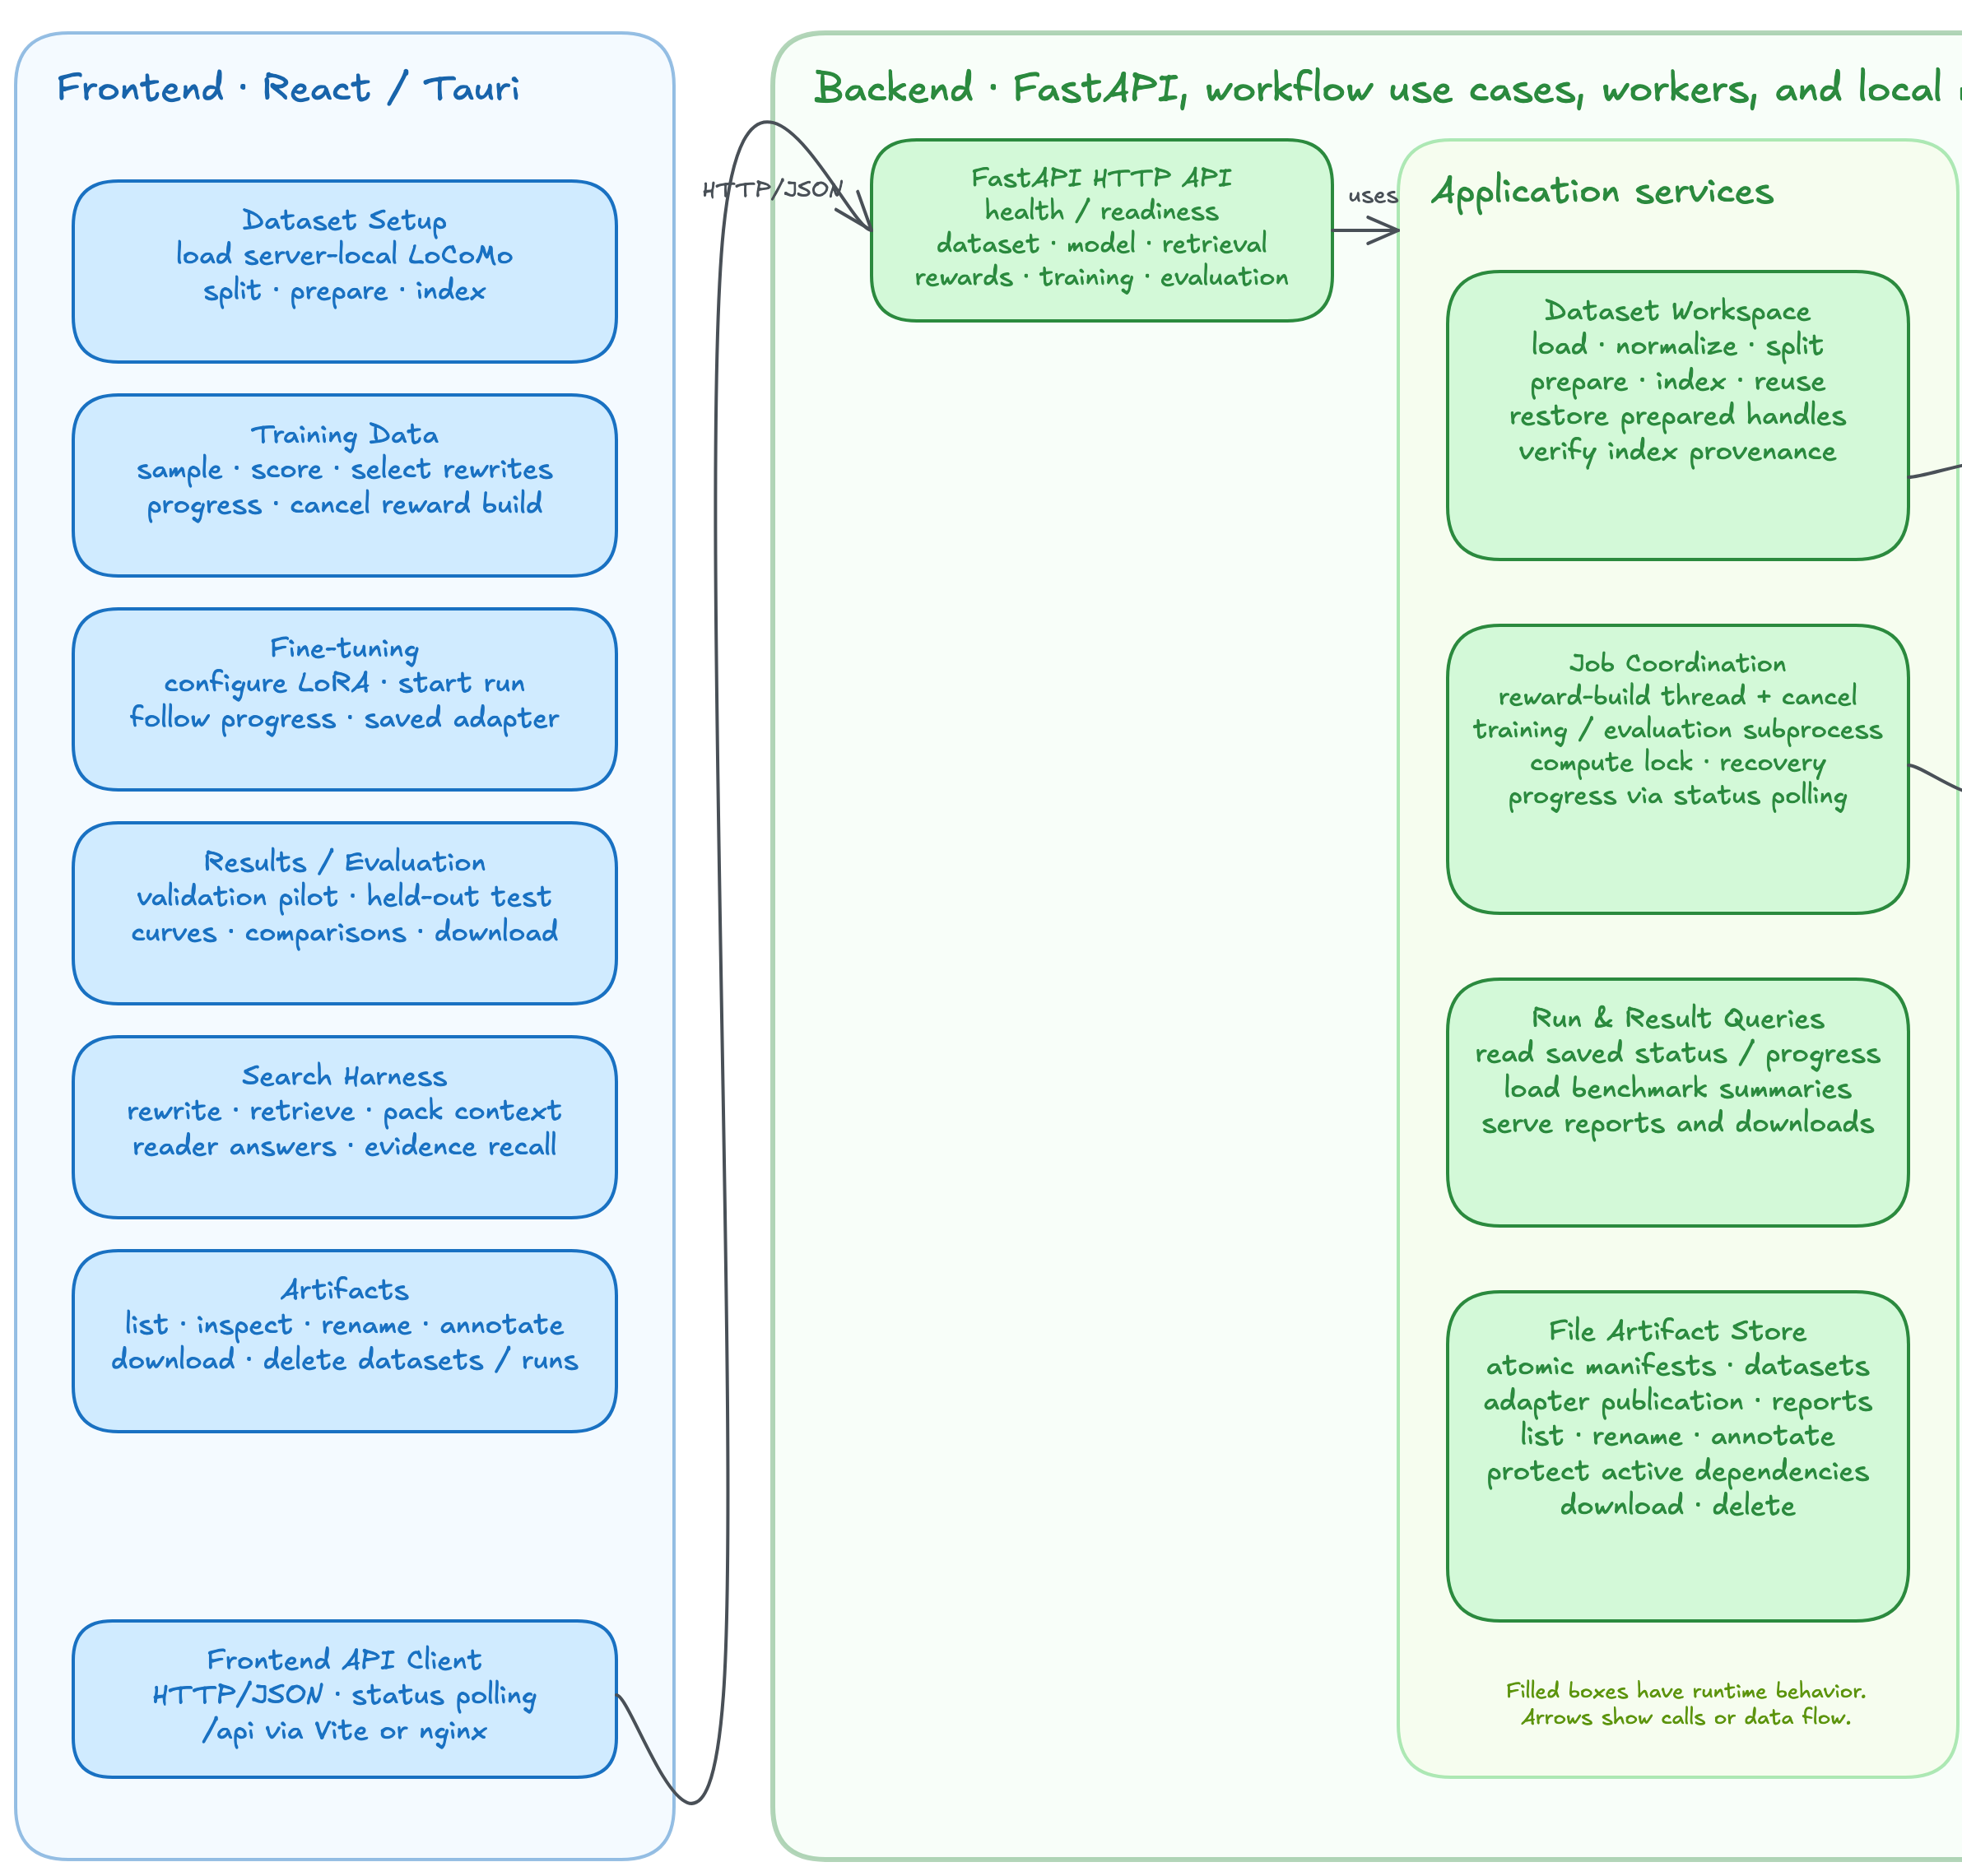
\includegraphics[height=5.43in]{figures/component-a.png}
\caption[Component architecture, part 1: console and application services]%
{Component architecture, part 1 of 3: the desktop console, the single HTTP
boundary, and the backend's application services. The console issues no
research decisions of its own. Arrows show calls or data flow; the backend
boundary and its heading continue into Figure~\ref{fig:component-b}.}
\label{fig:component-a}
\end{figure}

\begin{figure}[p]
\centering
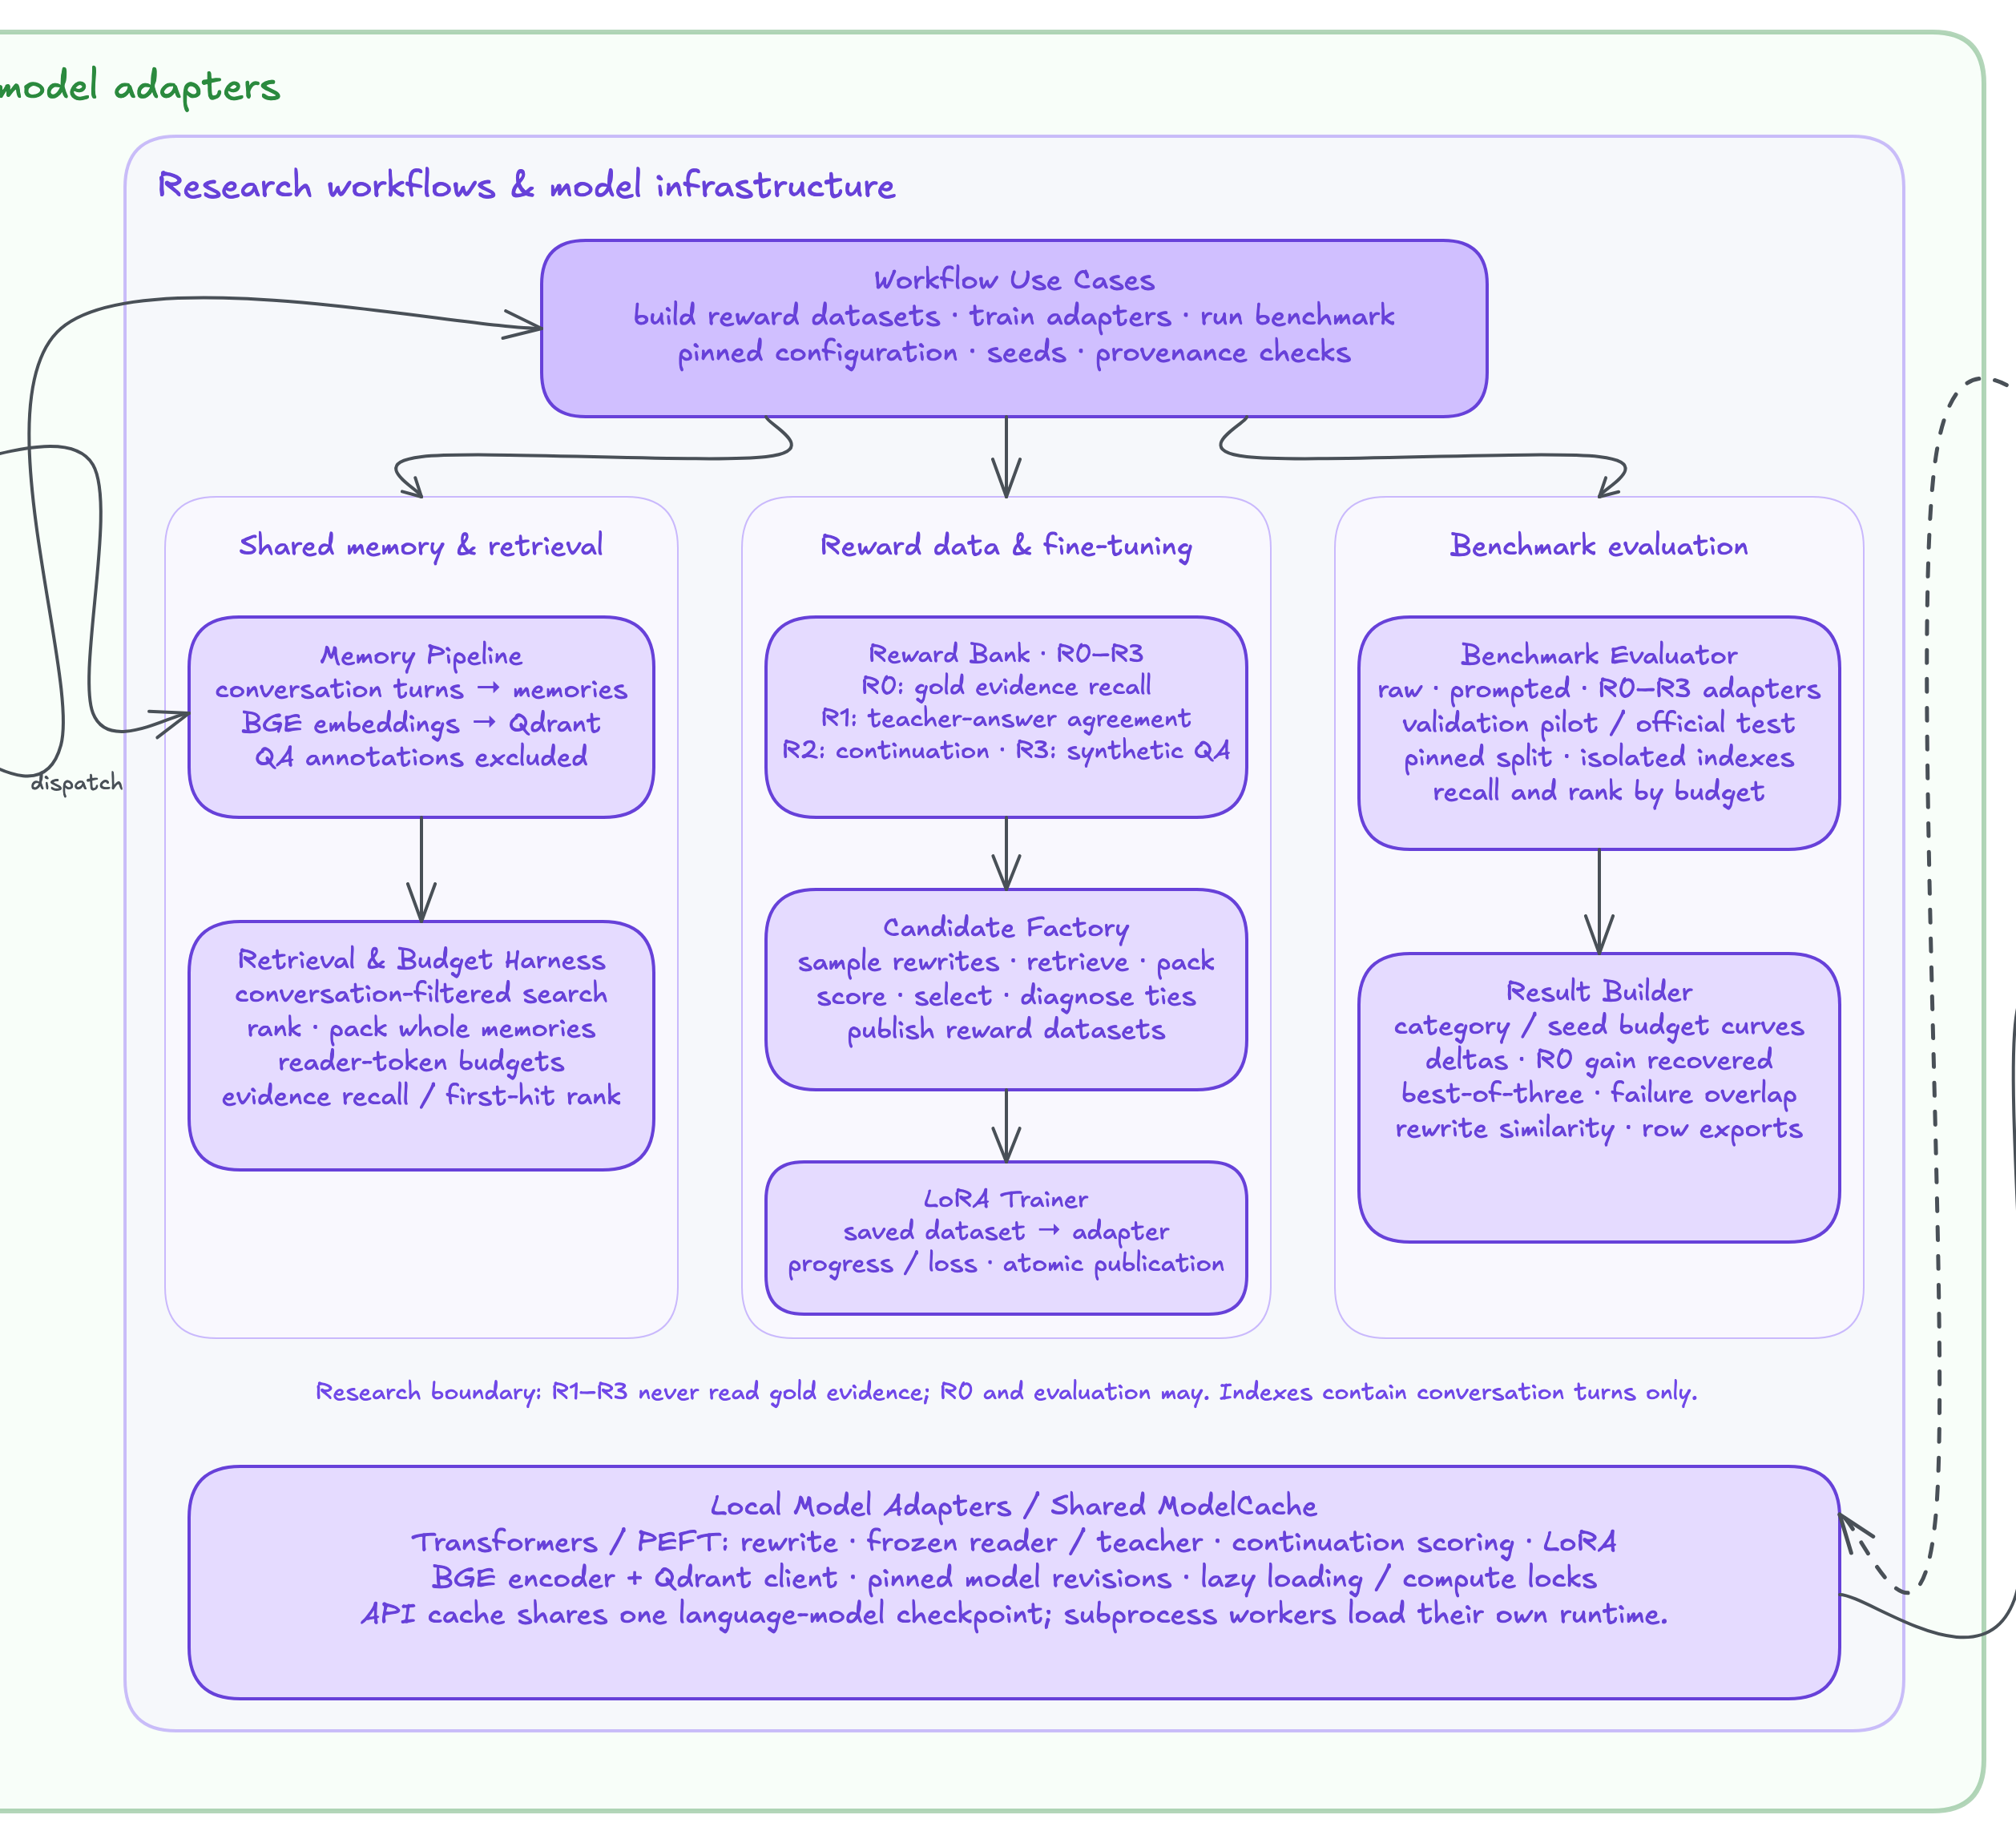
\includegraphics[height=5.43in]{figures/component-b.png}
\caption[Component architecture, part 2: research workflows and models]%
{Component architecture, part 2 of 3: the research workflows and model
infrastructure, continuing from Figure~\ref{fig:component-a}. The five research
components of Section~\ref{sec:highlevel} appear here, and the research
boundary across the middle records that \Ra--\Rc\ never read gold evidence
while \Rz\ and evaluation may.}
\label{fig:component-b}
\end{figure}

\begin{figure}[p]
\centering
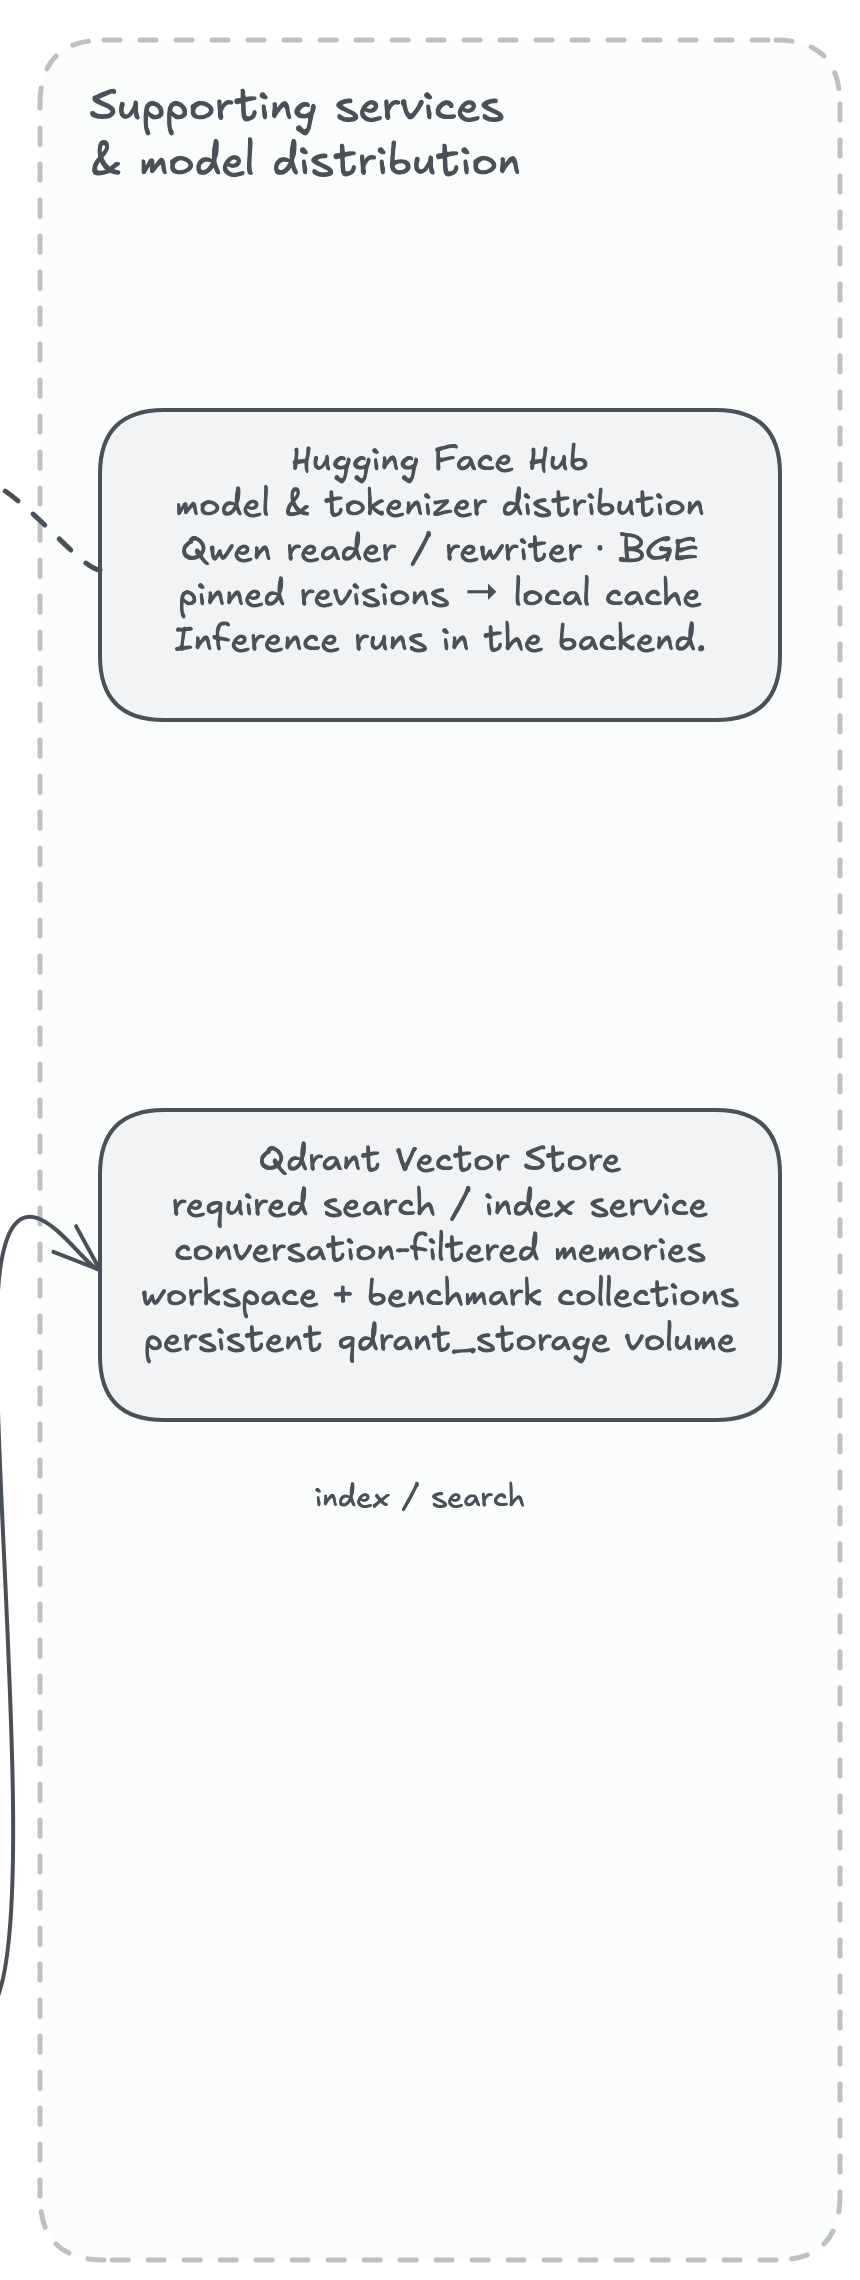
\includegraphics[height=7.1in]{figures/component-c.png}
\caption[Component architecture, part 3: the supporting services]%
{Component architecture, part 3 of 3: the two services the backend depends on,
continuing from Figure~\ref{fig:component-b}. Qdrant is required at run time;
the Hugging Face Hub is contacted only to fetch pinned model revisions into a
local cache, and all inference runs inside the backend. The arrows entering at
the left come from the model adapters in Figure~\ref{fig:component-b}.}
\label{fig:component-c}
\end{figure}

Five components carry the research logic, and each is independently testable.
The \emph{memory pipeline} converts conversations into memories, embeds them,
and indexes them. The \emph{retrieval and budget harness} issues a query,
ranks memories, packs them to a token budget, and scores the packed set. The
\emph{reward bank} holds the four scorers behind a single interface. The
\emph{candidate factory and training loop} samples rewrites, scores them,
assembles the winners into a fine-tuning set, and runs the fine-tune. The
\emph{benchmark evaluator} scores the whole ladder on a held-out split and
aggregates the results. Sections~\ref{sec:frozen} through \ref{sec:evaluator}
describe each in turn.

The backend follows a ports-and-adapters layering~\cite{cleanarch}. Domain
entities---\code{Conversation}, \code{Session}, \code{Turn}, \code{Memory},
\code{QA}---carry no framework dependencies. Application use cases depend only
on ports: \code{DatasetPort}, \code{EmbeddingPort},
\code{MemoryStorePort}, \code{LLMPort}, \code{RewriteTrainerPort}, and
\code{ArtifactStore}. Infrastructure supplies the concrete adapters: a LoCoMo JSON reader, a BGE encoder, a Qdrant
client, a Transformers generation and scoring adapter, and a PEFT LoRA trainer.
The practical payoff is that the reward bank, which is the contribution, is
written against interfaces and can be exercised with substituted models in
tests.

\section{The Frozen Harness}
\label{sec:frozen}

Freezing is the mechanism that makes the comparison valid, so it is worth being
precise about what is frozen and how that is enforced.

\subsection{Memory Construction}

A memory is one conversation turn. Rendering is deterministic: the session
timestamp in ISO~8601, the speaker, and the text, in the form
\code{[<timestamp>] <speaker>: <text>}. The memory identifier is a UUID~v5
derived from the conversation, session, and turn identifiers, so re-indexing
the same corpus produces the same identifiers and cannot silently duplicate
points. Only conversation turns are indexed; question-answer annotations are
never embedded. The rendering format carries an explicit version number so that
a change to it invalidates existing indexes rather than mixing formats.

This is intentionally the simplest possible memory construction. PPRO builds
episodic memories, semantic memories, and user profiles~\cite{ppro}; this
project builds none of those, because memory construction is held constant and
a simpler construction makes the baseline easier to reproduce.

\subsection{Encoder and Index}

The encoder is BGE-base-en-v1.5~\cite{bge} pinned to a specific commit,
768~dimensions, 512-token input limit, normalized outputs, run on CPU. Queries
receive BGE's retrieval instruction prefix; documents receive none. Weights are
frozen and never trained.

Vectors are stored in Qdrant~\cite{qdrant}, and search is filtered by
conversation identifier, so a query over one conversation can never retrieve
another user's memories. Every index record carries the corpus hash, the
embedding configuration, the memory format version, the collection, and the
vector size, and points carry the matching signature. On startup and before
reuse the system verifies the expected identifiers, payloads, dimensions, and
per-conversation counts; an index that is missing, altered, incompatible, or
partially written is not advertised as ready. This matters more than it may
appear: a silently stale index would corrupt every number in
Chapter~\ref{ch:methodology} while leaving the system apparently healthy.

\subsection{Retrieval, Packing, and the Budget}

Retrieval returns the top $k=20$ memories for a query within a conversation.
Packing then walks that ranked list in order and admits whole memories while
the running total fits the token budget, stopping at the first memory that
would overrun it. Memories are never truncated, because a half-memory would
make evidence recall ambiguous. Tokens are counted in the reader's own
tokenizer, which is the only count that corresponds to what the reader can
actually accept.

Budgets of 128, 256, 512, 1024, and 2048 reader tokens are evaluated. Because a
single search can be packed at every budget, the whole curve costs one search.
Reporting a curve rather than a single number is a deliberate choice: a method
that wins only when the budget is generous tells a different story from one
that wins everywhere, and real deployments differ widely in the context they
can afford.

\subsection{Reader and Rewriter}

Both roles are filled by Qwen2.5-0.5B~\cite{qwen} pinned to a specific commit.
One frozen checkpoint serves as the reader for \Ra, the continuation scorer for
\Rb, the question generator for \Rc, and the base model for every fine-tune. A
process-wide model cache holds one copy per checkpoint, and construction is
serialized so that a second request joins the first load rather than starting
its own.

Using a 0.5B model is the most significant departure from the project proposal,
which anticipated a model of roughly 10B parameters trained with LoRA on a
16~GiB GPU. Section~\ref{sec:deviations} records the reasoning and the
consequences.

\section{The Reward Bank}
\label{sec:rewards}

The reward bank is the contribution. All four scorers implement one interface:
given a packed context, return a scalar. A builder for each reward turns a
partition of the corpus into a stream of scoring inputs, where each input
carries the text to be rewritten, the conversation to search, a scoring
function, and optionally a restriction on which turns are eligible to be
retrieved. Swapping the training signal is therefore a configuration change
rather than a code change, which is what makes the comparison in
Chapter~\ref{ch:methodology} a controlled one.

Figure~\ref{fig:rewards} shows what each reward consumes and what it computes.

\begin{figure}[htbp]
\centering
\begin{singlespace}
\begin{tikzpicture}[
  font=\footnotesize,
  box/.style={draw,rounded corners=2pt,align=center,inner sep=3pt,
              text width=1.2in},
  hdr/.style={box,fill=black!8,font=\footnotesize\bfseries,minimum height=8.5mm},
  src/.style={box,fill=blue!6,draw=blue!50,minimum height=8.5mm},
  mid/.style={box,minimum height=8.5mm},
  calc/.style={box,fill=green!6,draw=green!45!black,minimum height=12mm},
  res/.style={box,fill=orange!8,draw=orange!60!black,minimum height=8.5mm},
  gold/.style={box,fill=red!7,draw=red!55},
  ar/.style={-{Stealth[length=1.5mm]},draw=black!60,shorten >=0.5pt}
]
% Column centres. Rows are aligned with the (col |- row) trick so that a taller
% cell in one column cannot push its neighbours out of line.
\def\cs{1.42in}
\node[hdr] (h1) at (0,0)      {R1\\full-context teacher};
\node[hdr] (h2) at (\cs,0)    {R2\\masked-turn prediction};
\node[hdr] (h3) at (2*\cs,0)  {R3\\synthetic evidence};
\node[hdr] (h4) at (3*\cs,0)  {R0\\supervised ceiling};

\node[src,below=3mm of h1] (s1) {reads: conversation\\+ training question};
\node[src]  (s2) at (h2 |- s1) {reads: conversation\\only};
\node[src]  (s3) at (h3 |- s1) {reads: conversation\\only};
\node[gold,minimum height=8.5mm] (s4) at (h4 |- s1)
      {reads: conversation\\+ \textbf{gold evidence}};

\node[mid,below=3mm of s1] (i1) {rewrites:\\the question};
\node[mid]  (i2) at (h2 |- i1) {rewrites:\\3 prior turns};
\node[mid]  (i3) at (h3 |- i1) {rewrites:\\a generated question};
\node[mid]  (i4) at (h4 |- i1) {rewrites:\\the question};

\node[calc,below=3mm of i1] (c1)
      {answer once from context,\\once from the whole\\conversation};
\node[calc] (c2) at (h2 |- c1)
      {predict the hidden turn\\with and without\\the context};
\node[calc] (c3) at (h3 |- c1)
      {is the source turn\\in the context?};
\node[gold,minimum height=12mm] (c4) at (h4 |- c1)
      {how many gold turns\\are in the context?};

\node[res,below=3mm of c1] (r1) {token-F1 of the\\two answers};
\node[res]  (r2) at (h2 |- r1) {log-likelihood\\\emph{gain}};
\node[res]  (r3) at (h3 |- r1) {1.0 or 0.0};
\node[gold,minimum height=8.5mm] (r4) at (h4 |- r1) {evidence recall};

\foreach \srcn/\dstn in {h1/s1,s1/i1,i1/c1,c1/r1, h2/s2,s2/i2,i2/c2,c2/r2,
                         h3/s3,s3/i3,i3/c3,c3/r3, h4/s4,s4/i4,i4/c4,c4/r4}
  \draw[ar] (\srcn) -- (\dstn);

\begin{scope}[on background layer]
  \node[draw=green!45!black,dashed,rounded corners=3pt,inner sep=6pt,
        fit=(h1)(r3)] (lf) {};
\end{scope}
\node[font=\scriptsize\itshape,green!35!black,anchor=north]
  at ([yshift=-1.5mm]lf.south) {label-free: never reads an annotation};
\node[font=\scriptsize\itshape,red!55!black,anchor=north,text width=1.2in,
      align=center] at ([yshift=-3mm]r4.south) {reads annotations\\by design};
\end{tikzpicture}
\end{singlespace}
\caption[The four reward signals]{The four reward signals. The three on the left derive their score
from the conversation alone; only \Rz\ reads the gold evidence annotations,
and it does so in order to serve as the ceiling.}
\label{fig:rewards}
\end{figure}

\subsection{\Ra: Full-Context Teacher}

A LoCoMo conversation fits in a modern context window. \Ra\ exploits that
directly: the same question is answered twice by the same frozen reader, once
from the memories the candidate query retrieved and once from the entire
conversation. The reward is the token-level F1 between the two answers, the
standard overlap measure from extractive question answering~\cite{squad}.

The full-conversation answer is the teacher, and it is free only because
personal memory is small. The teacher answer is computed once per question and
cached across all candidates for that question, so the cost is one extra
long-context generation per question rather than one per candidate. Two
conditions make an input ineligible rather than wrong: if the full conversation
does not fit the reader's window, the input is skipped as
\code{full\_history\_too\_long}; if the teacher declines to answer, it is
skipped as \code{teacher\_abstained}. A candidate whose packed context is empty
scores zero, and a candidate whose own context overruns the window skips the
input.

AdaQR~\cite{adaqr} is the nearest prior work, and the difference is
instructive. AdaQR scores a rewrite by the marginal probability a reader
assigns to the conversational answer; it must, because its corpus is too large
to read. \Ra's teacher sees the entire store. The signal is therefore stronger,
and it is available only in the memory setting.

\subsection{\Rb: Masked-Turn Prediction}

\Rb\ removes questions from the problem entirely. A turn is hidden, a query is
built from the three turns preceding it, and the reward is the increase in the
frozen model's log-likelihood of the hidden turn when the retrieved memories
are prepended to those three turns. Formally, with $c$ the packed context, $p$
the prior turns, and $t$ the hidden turn, the reward is
$\log P(t \mid c, p) - \log P(t \mid p)$.

Subtracting the no-context baseline is what makes the signal meaningful. The
absolute likelihood of a turn is dominated by how predictable that turn is in
general, which has nothing to do with the query; the difference isolates the
contribution of what was retrieved. The baseline is computed once per input and
cached. Retrieval is restricted to turns strictly earlier than the hidden one,
which prevents the trivial solution of retrieving the answer itself.

There are no questions, no answers, and no annotations anywhere in this
signal---the conversation supervises itself. It is also the cheapest of the
three, since scoring a continuation is a single forward pass with no
generation.

\subsection{\Rc: Synthetic Evidence}

\Rc\ manufactures the annotations that \Rz\ reads. A turn is selected, the
frozen model is prompted to write a standalone question that the turn answers,
and the pair is kept. The reward is binary: $1.0$ if the packed context
contains the source turn, $0.0$ otherwise. Generated questions are validated
before use---a question must parse, must terminate in a question mark, and must
not refer to ``this statement'' or ``the passage''---and failures are recorded
as \code{invalid\_synthetic\_question} rather than silently dropped. The
closest prior work is RL-QR's index-aligned synthetic queries~\cite{rlqr}, and
the technique is the inverse of doc2query~\cite{doc2query}; the validation step
borrows the filtering discipline of Self-Instruct~\cite{selfinstruct}.

\Rc\ is included partly because it has a known weakness. A question generated
from a message tends to reuse that message's vocabulary, which produces exactly
the easy case where a rewriter adds least. Predicting that \Rc\ underperforms
is cheap; measuring by how much, and on which question categories, is the
useful result.

\subsection{\Rz: Supervised Ceiling}

\Rz\ reproduces the retrieval half of PPRO's reward: a candidate scores the
fraction of the annotated evidence turns for its question that appear among the
packed memories. PPRO's second term, the similarity of the resulting answer to
a reference answer, is deliberately omitted, because it grades the wording of
an answer rather than the behavior of a query, and because scoring generated
text by reference similarity is the practice the evaluation literature argues
against~\cite{hownot}.

\Rz\ is not a competitor. It is trained with the same procedure, the same
candidate budget, the same base model, and the same hyperparameters as the
other three, so that the only difference between \Rz\ and a label-free reward
is the information the reward consumes. Every label-free result in
Chapter~\ref{ch:methodology} is reported both absolutely and as a fraction of
\Rz.

\subsection{What Each Reward Requires}

Table~\ref{tab:rewards} summarizes the inputs each reward consumes. All four
train on the same corpus and the same partition, so the reward is the only
variable; what differs is which part of that corpus each one reads.

\begin{table}[htbp]
\caption[Inputs consumed by each reward]{Inputs consumed by each reward. Only \Rz\ reads the evidence
annotations. The corpus must nonetheless be an annotated one, because
evaluation scores every configuration against those annotations.}
\label{tab:rewards}
\centering
\begin{tab}
\begin{tabular}{@{}L{0.6in}L{1.2in}C{0.8in}C{0.62in}L{1.72in}@{}}
\toprule
\textbf{Reward} & \textbf{Signal} & \textbf{Questions?} &
\textbf{Labels?} & \textbf{Skip reasons} \\
\midrule
\Ra & Agreement between retrieved-context and full-context answers &
Yes & No & \skid{full\us history\us too\us long,\newline teacher\us abstained,\newline retrieved\us context\us too\us long} \\
\Rb & Log-likelihood gain on a hidden turn & No & No &
\skid{blank\us hidden\us turn,\newline prediction\us baseline\us too\us long,\newline prediction\us context\us too\us long} \\
\Rc & Retrieval of a self-generated question's source turn & No &
No & \skid{blank\us source\us turn,\newline invalid\us synthetic\us question} \\
\Rz & Recall of annotated evidence turns & Yes & \textbf{Yes} &
\skid{missing\us conversation,\newline invalid\us question,\newline missing\us evidence,\newline unresolved\us evidence} \\
\bottomrule
\end{tabular}
\end{tab}
\end{table}

Skip reasons are not incidental. A reward that silently discards hard inputs
would flatter itself, so every attempted input produces either a kept example
or a recorded reason, and the histogram of reasons is published with the
dataset. Section~\ref{sec:results} reports those histograms alongside the
recall numbers.

\section{Candidate Factory and Training Loop}
\label{sec:loop}

Figure~\ref{fig:pipeline} shows the path from a training input to a trained
adapter. The loop is the same for all four rewards; only the scorer differs.

\begin{figure}[htbp]
\centering
\begin{singlespace}
\begin{tikzpicture}[
  font=\footnotesize,
  node distance=4mm,
  stage/.style={draw,rounded corners=2pt,align=center,inner sep=4pt,
                minimum height=9mm,text width=1.02in},
  frozen/.style={stage,fill=blue!6,draw=blue!50},
  work/.style={stage,fill=green!6,draw=green!45!black},
  train/.style={stage,fill=orange!10,draw=orange!65!black},
  ar/.style={-{Stealth[length=1.7mm]},draw=black!65}
]
\node[stage,fill=black!5] (inp) {training input\\(question or turns)};
\node[train,right=6mm of inp] (rw) {rewriter LM\\sample $k{=}8$, $T{=}0.7$};
\node[stage,right=6mm of rw] (cand) {candidate\\queries $q_1 \dots q_k$};

\node[frozen,below=7mm of cand] (emb) {BGE encode\\(frozen)};
\node[frozen,left=6mm of emb] (qd) {Qdrant search\\top-$k{=}20$};
\node[frozen,left=6mm of qd] (pack) {pack to\\512 tokens};

\node[work,below=7mm of pack] (score) {reward scorer\\\Rz/\Ra/\Rb/\Rc};
\node[work,right=6mm of score] (sel) {select argmax\\skip if all tied};
\node[train,right=6mm of sel] (ds) {reward dataset\\(prompt, rewrite)};

\node[train,below=7mm of ds] (sft) {LoRA SFT\\$r{=}8$, $\alpha{=}16$};
\node[stage,fill=orange!18,draw=orange!70!black,left=6mm of sft] (ad)
  {trained\\adapter};

\draw[ar] (inp) -- (rw);
\draw[ar] (rw) -- (cand);
\draw[ar] (cand) -- node[right,font=\scriptsize,xshift=1pt]{each $q_i$} (emb);
\draw[ar] (emb) -- (qd);
\draw[ar] (qd) -- (pack);
\draw[ar] (pack) -- (score);
\draw[ar] (score) -- (sel);
\draw[ar] (sel) -- (ds);
\draw[ar] (ds) -- (sft);
\draw[ar] (sft) -- (ad);

\begin{scope}[on background layer]
  \node[draw=blue!50,dashed,rounded corners=3pt,inner sep=4pt,
        fit=(pack)(emb)] (fz) {};
\end{scope}
\node[font=\scriptsize\itshape,blue!55!black,anchor=west]
  at ([xshift=2mm]fz.east) {frozen for every configuration};
\end{tikzpicture}
\end{singlespace}
\caption[The candidate factory and training loop]{The candidate factory and training loop. Sampling, scoring, and
selection run offline; only the rewriter changes between configurations.}
\label{fig:pipeline}
\end{figure}

\subsection{Candidate Generation}

For each input, the rewriter samples eight candidates at temperature~0.7 with a
48-token limit, and duplicates are removed case-insensitively, so fewer than
eight distinct candidates is normal and expected. Each candidate's random seed
is derived deterministically by hashing the run seed, the input identifier, and
the candidate index, which means the same three values always reproduce the
same candidate set. Determinism at this level of granularity is what makes a
failed run resumable and a surprising number reproducible.

\subsection{Selection}

Candidates are scored, and the first candidate attaining the maximum score is
kept. Two situations produce no training example and are recorded rather than
hidden. If fewer than two distinct candidates survive deduplication, the input
is skipped as \code{too\_few\_candidates}. If every candidate receives the same
score, the input is skipped as \code{all\_scores\_tied}---a tie carries no
preference, and training on an arbitrary member of a tie would inject noise
presented as signal. An option exists to retain one rewrite when every
candidate achieves perfect evidence recall under \Rz, since that particular tie
reflects an easy question rather than an uninformative reward; it is disabled
in the frozen benchmark configuration.

\subsection{Fine-Tuning}

Kept pairs are written as prompt-and-completion rows and fine-tuned with
LoRA~\cite{lora} at rank~8 and $\alpha=16$, one epoch, learning rate
$2\times10^{-4}$, batch size~1 with four gradient accumulation steps, and a
512-token maximum length. Rows that do not fit the token limit are excluded and
counted. Adapters are published atomically: training writes to a staging
directory, and the artifact is moved into place and hashed only on success, so
an interrupted run cannot leave a half-written adapter that a later evaluation
would silently load.

At serving time the rewriter sees only the user's message. The conversation,
the teacher, the hidden turns, and the annotations exist only during offline
training. This asymmetry is the point of the design: expensive signals are
affordable offline, and none of them is required online.

\section{The Benchmark Evaluator}
\label{sec:evaluator}

Evaluation is a separate workflow with its own index. The held-out partition is
indexed into a dedicated Qdrant collection so that test memories are never
mixed with the training collection. Six configurations plus two diagnostics are
scored on every eligible question at every budget.

For each question and configuration, the evaluator produces the query---the raw
message, or a greedy rewrite from the relevant model---searches, packs at each
budget, and records recall, the rank of the first evidence hit, the tokens
used, the matched turn identifiers, and whether the rewrite came back empty. An
empty rewrite falls back to the original query and is counted, rather than
being dropped, because a model that sometimes emits nothing has a real defect
that a drop would hide. Rewriting at evaluation time uses temperature~0, so the
measured configuration is deterministic even though training used sampling.

Two diagnostic series accompany the ladder. The \emph{gold query} series builds
a query by concatenating the annotated evidence turns themselves; it is not a
method, since it reads the answer, but it bounds what any query could retrieve
and therefore reports the headroom available. The \emph{best-of-three} series
takes, per question, the best of the three label-free results; it is likewise
not a method, since choosing it requires knowing the outcome, but it quantifies
how much the three signals are complementary rather than redundant.

Aggregation produces per-seed rows and then curves averaged across seeds with
standard deviations, broken out by category and budget. Derived quantities
include the delta against the raw baseline, the delta against the prompted
baseline, the ratio to \Rz, and the fraction of \Rz's gain recovered, defined
as
\[
  \text{gain recovered} \;=\;
  \frac{\text{recall}_{\text{reward}} - \text{recall}_{\text{prompted}}}
       {\text{recall}_{\Rz} - \text{recall}_{\text{prompted}}},
\]
reported only where \Rz\ improves on the prompted baseline, since the ratio is
meaningless otherwise. The evaluator also computes the overlap of zero-recall
failures across the three label-free rewards and the pairwise lexical
similarity of their rewrites, which together answer whether the signals differ
in substance or only in name.

A run is admitted as \emph{official} only if it satisfies a set of provenance
checks: all three seeds present, each with a completed adapter for each of
\Rz--\Rc; every adapter trained on the benchmark corpus hash, split, and
training conversations; identical reward-build and fine-tuning settings;
matching recorded training device and precision; a recorded peak device-memory
figure within the 16~GiB target; and adapter file hashes matching those
recorded at publication. Runs that fail any check are rejected rather than
reported with a caveat.

\section{Implementation}
\label{sec:implementation}

Figures~\ref{fig:module-a} through~\ref{fig:module-c} show the module structure
of the implemented system. The dashed arrows running upward from infrastructure
to the application ports in Figure~\ref{fig:module-b} are the dependency
inversion the design rests on: each adapter implements a port that the use
cases depend on, so no use case names a concrete model, store, or file format.

\begin{sidewaysfigure}
\centering
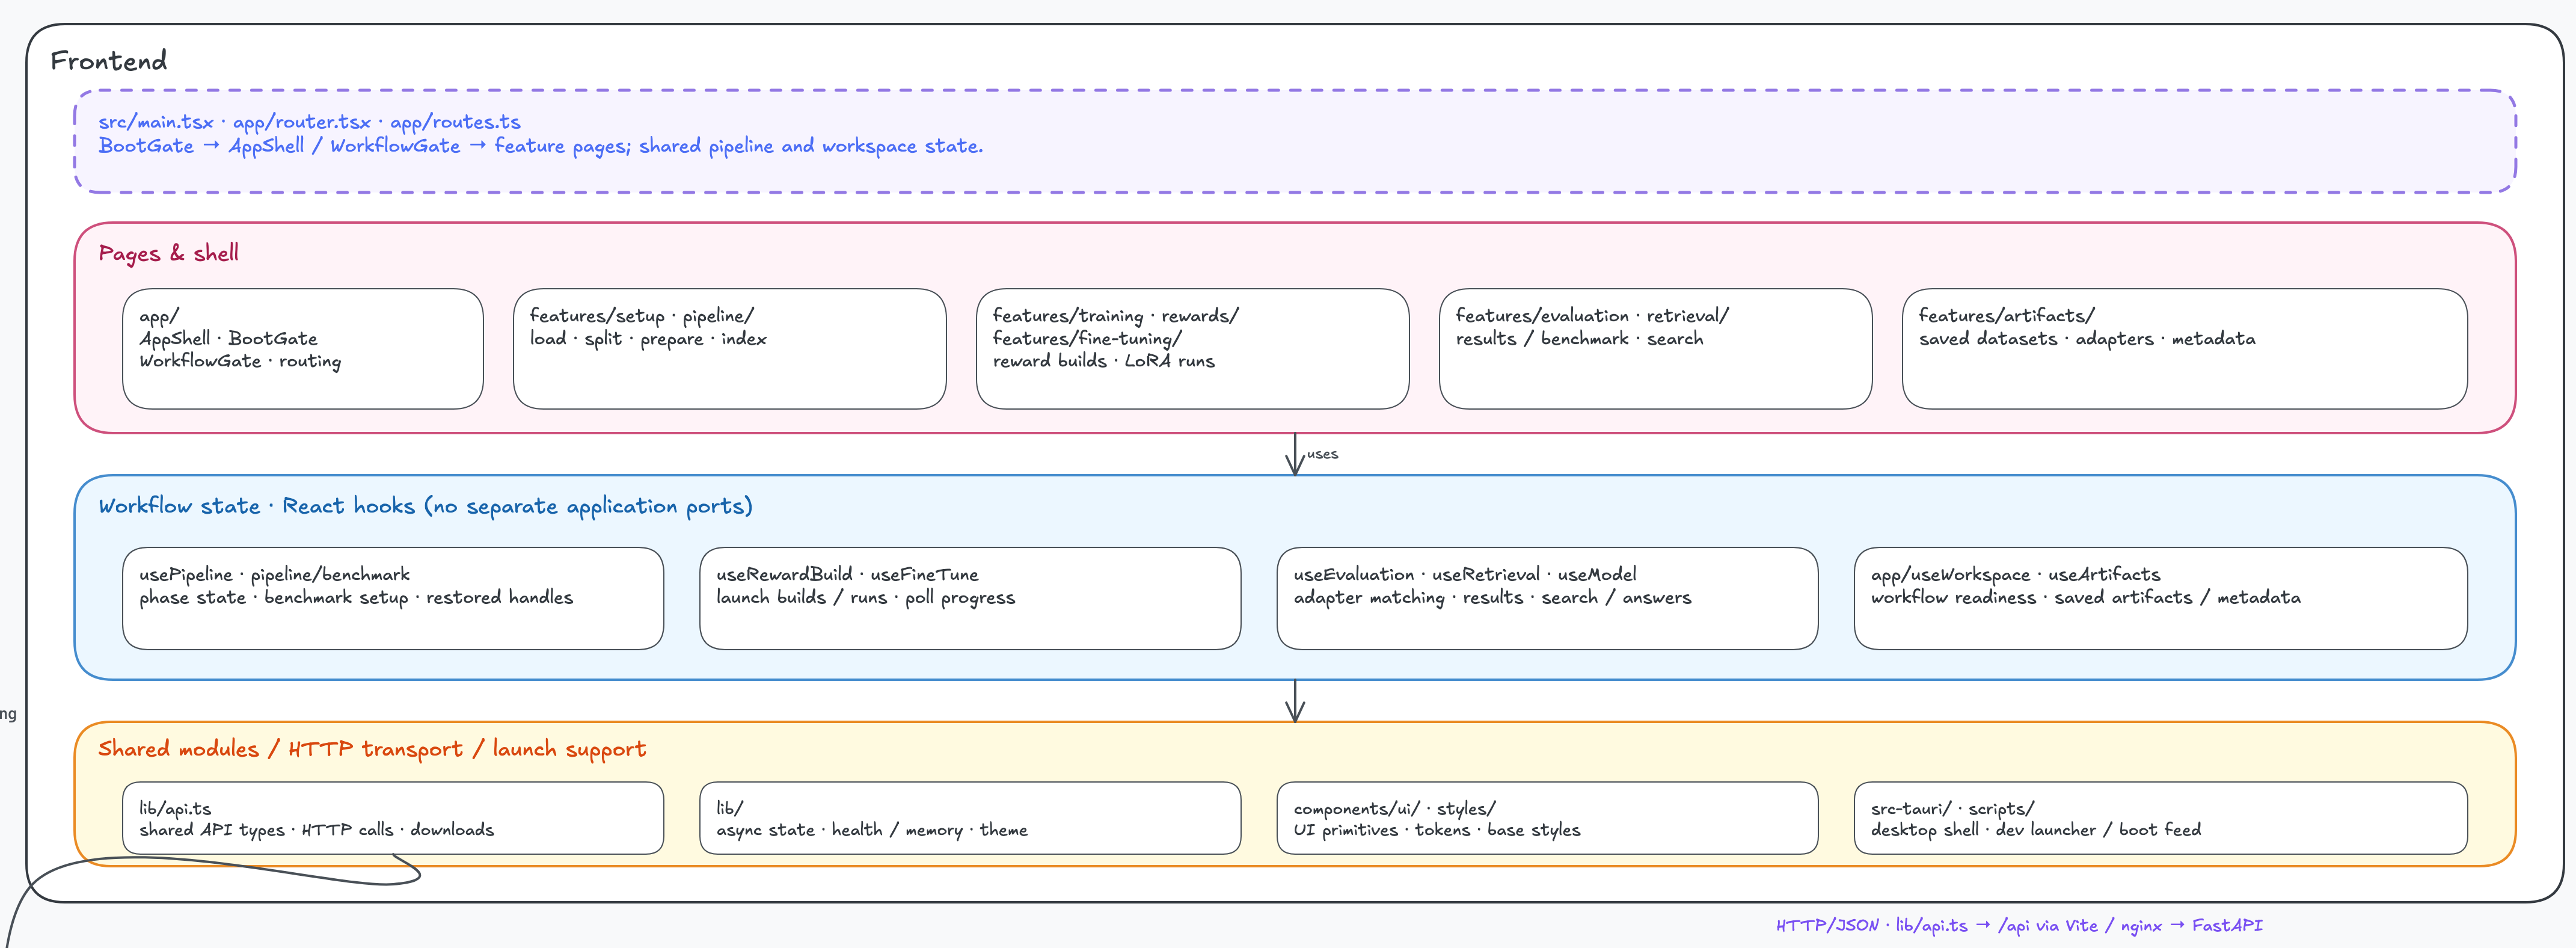
\includegraphics[width=8.8in]{figures/module-a.png}
\caption[Module structure, part 1: the frontend]%
{Module structure, part 1 of 3: the frontend. Pages and shell sit above the
workflow-state hooks, which sit above the shared modules and HTTP transport.
Throughout Figures~\ref{fig:module-a}--\ref{fig:module-c}, solid arrows are
calls, dashed arrows mark a port implemented by an adapter, dashed boxes are
composition and wiring, and coloured bands group layers.}
\label{fig:module-a}
\end{sidewaysfigure}

\begin{sidewaysfigure}
\centering
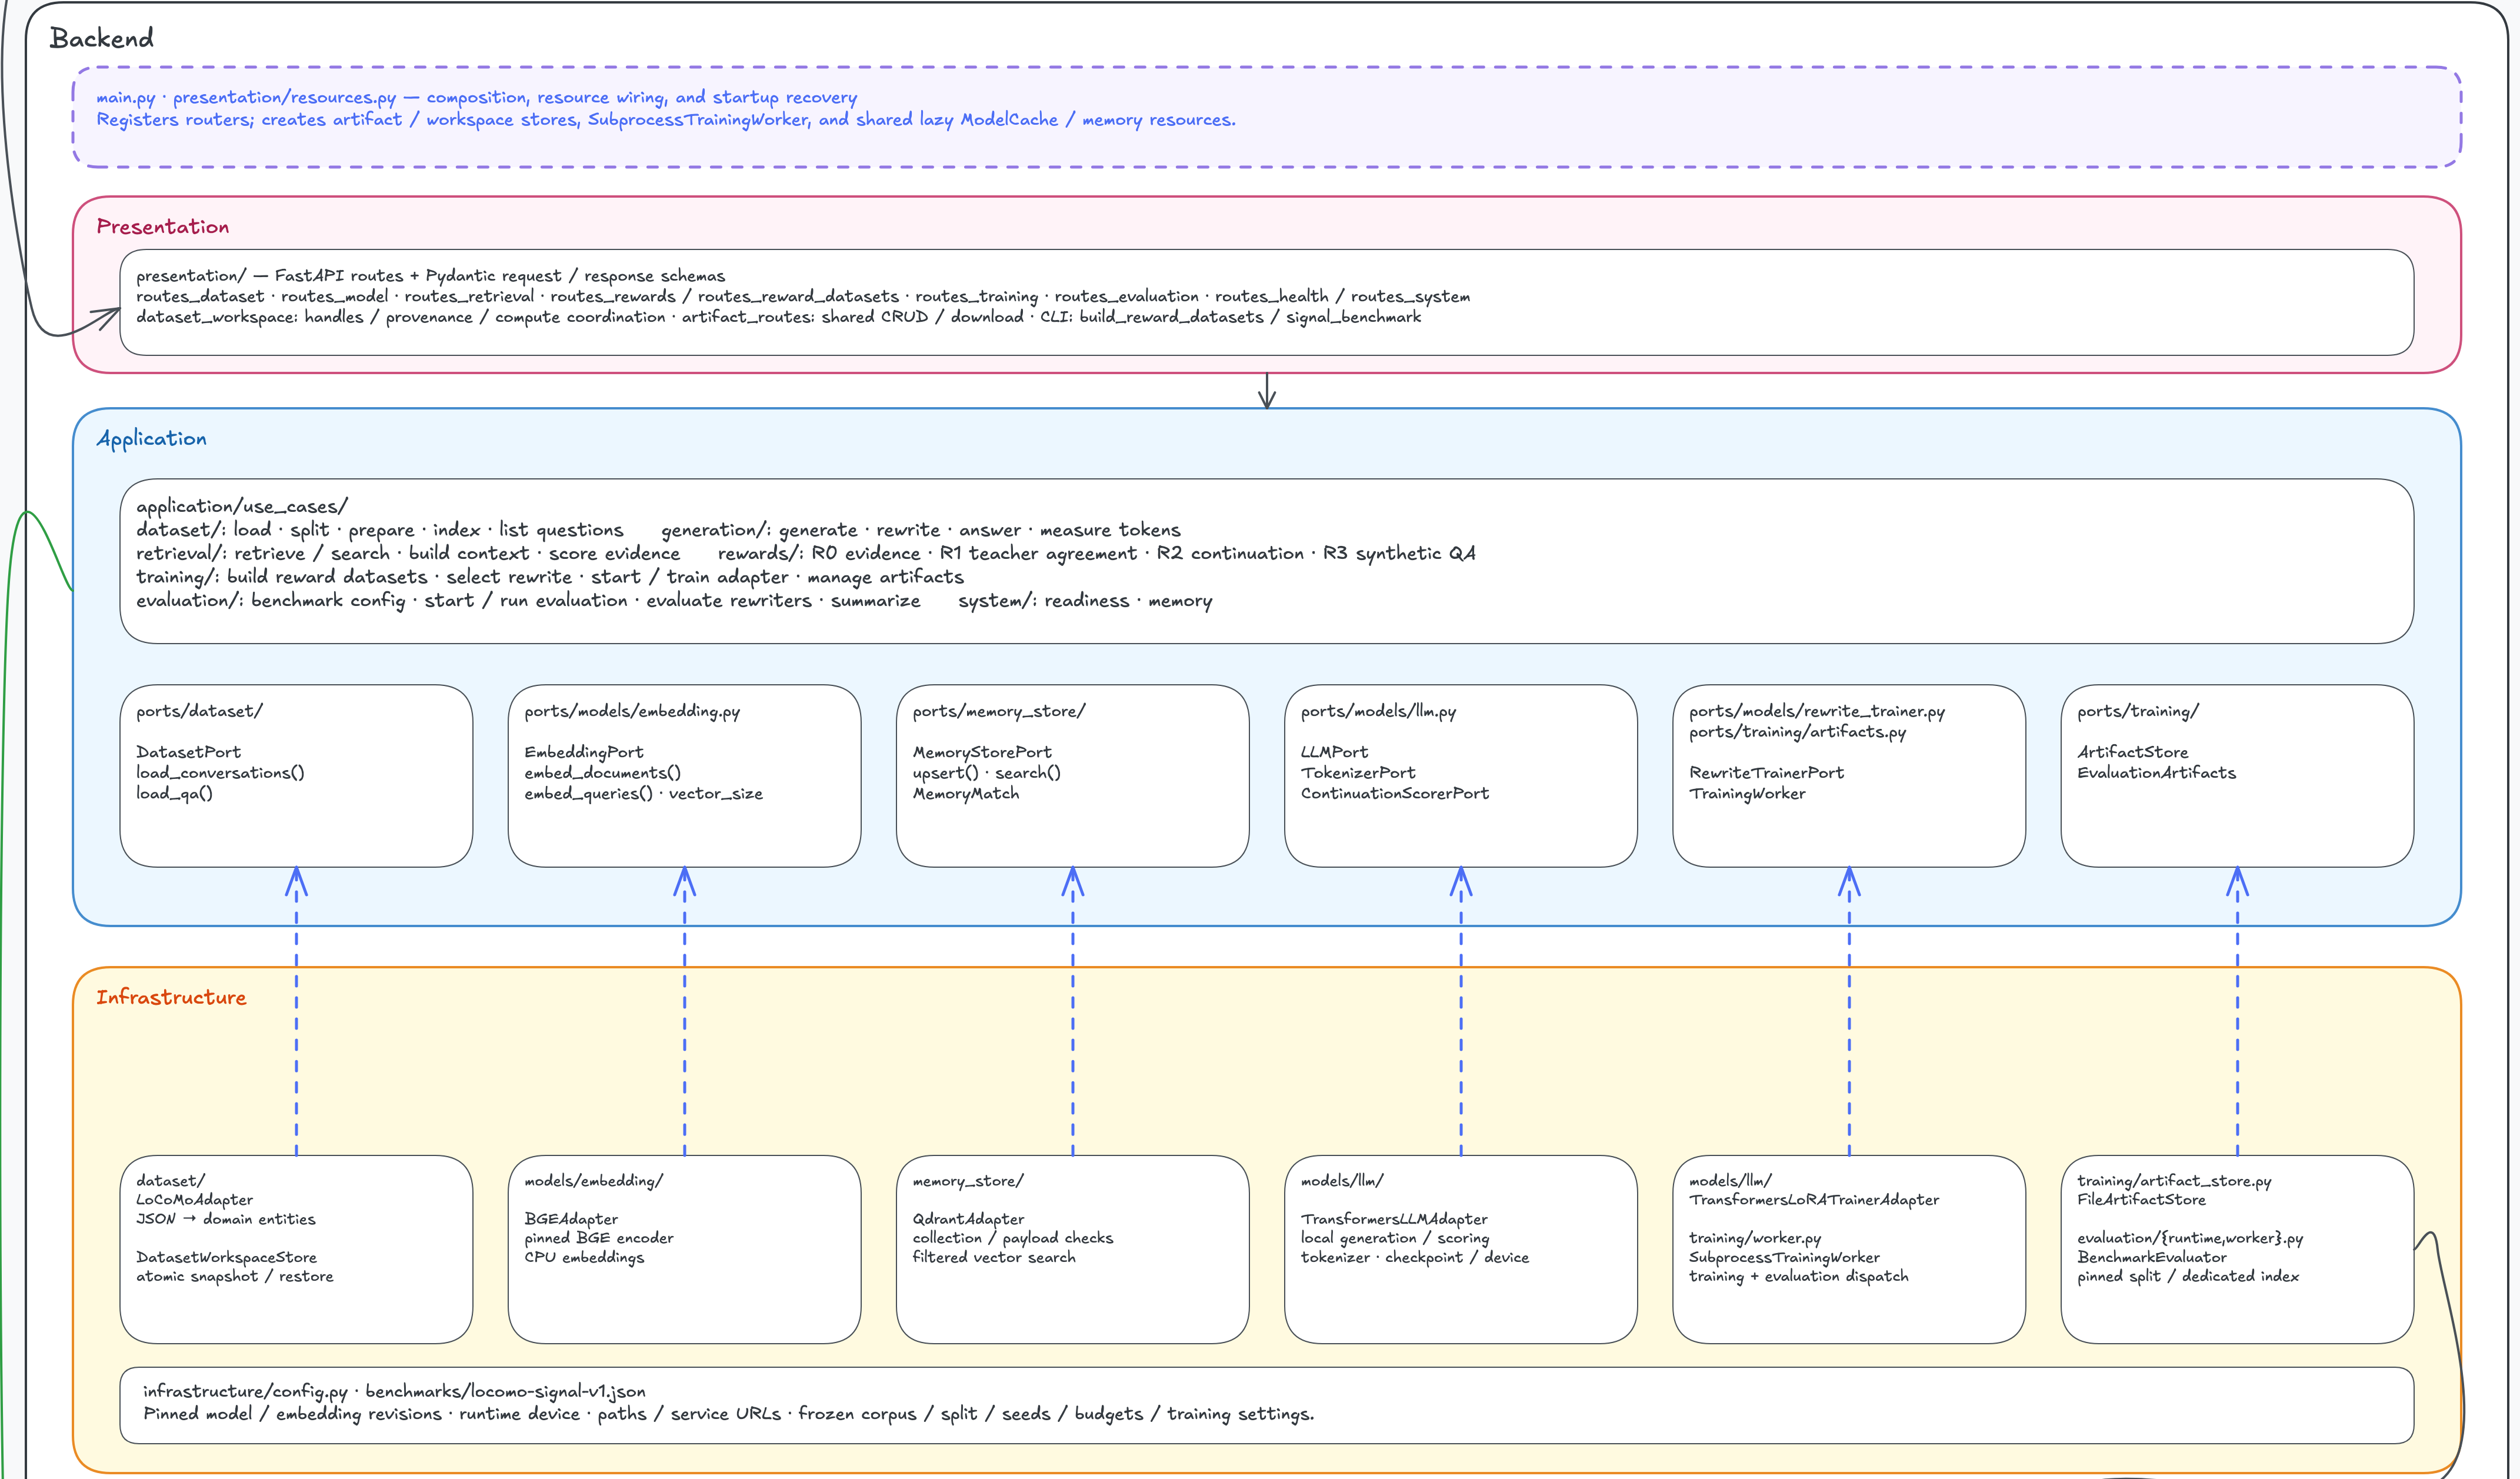
\includegraphics[width=8.8in]{figures/module-b.png}
\caption[Module structure, part 2: the backend layers]%
{Module structure, part 2 of 3: the backend's composition root, presentation,
application, and infrastructure layers, continuing from
Figure~\ref{fig:module-a}.}
\label{fig:module-b}
\end{sidewaysfigure}

\begin{sidewaysfigure}
\centering
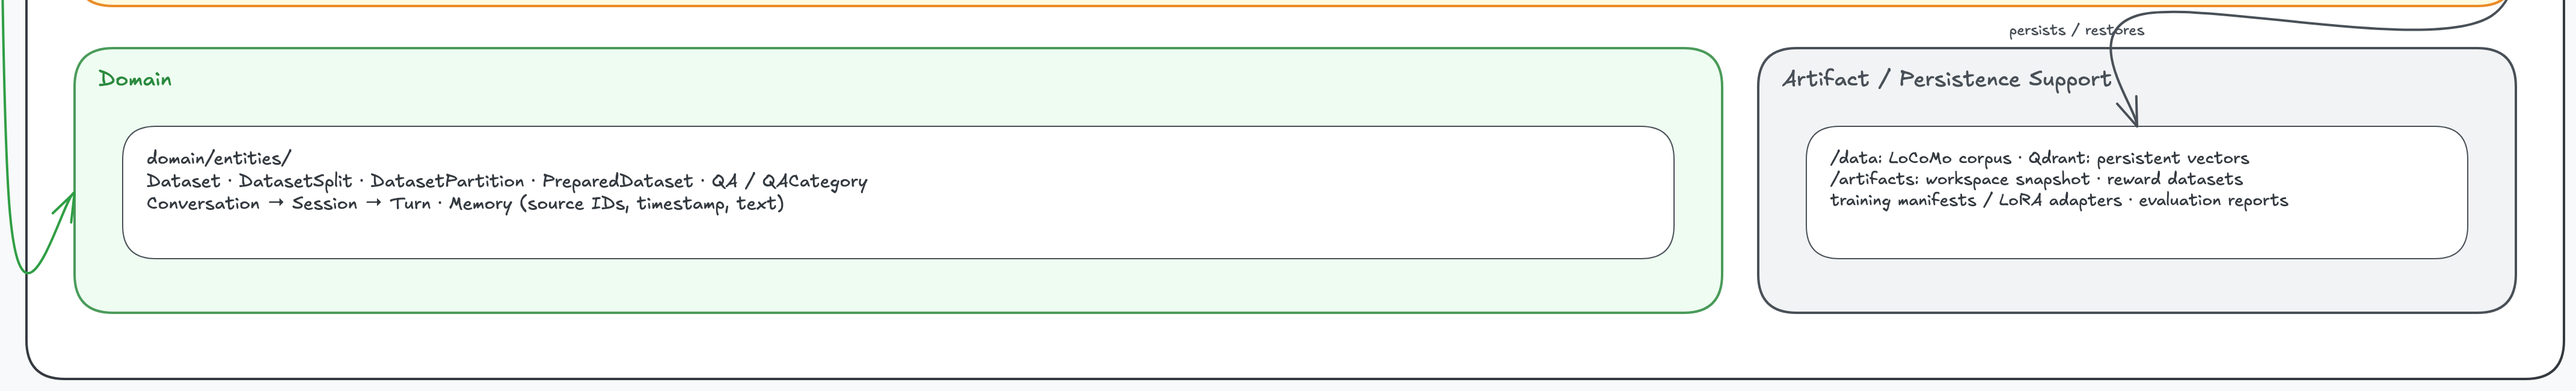
\includegraphics[width=8.8in]{figures/module-c.png}
\caption[Module structure, part 3: domain and persistence]%
{Module structure, part 3 of 3: the domain entities and the artifact and
persistence support, continuing from Figure~\ref{fig:module-b}. Domain entities
carry no framework dependencies, and every durable artifact---the workspace
snapshot, reward datasets, training manifests, LoRA adapters, and evaluation
reports---is written beneath a single artifacts root.}
\label{fig:module-c}
\end{sidewaysfigure}

\subsection{Backend}

The backend is a FastAPI application of roughly 100~Python modules organized
into the four layers of Section~\ref{sec:highlevel}. Use cases are grouped by
concern: \code{dataset} (load, split, prepare, index, list questions),
\code{generation} (generate, rewrite, answer, measure tokens),
\code{retrieval} (search, build context, score evidence), \code{rewards}
(the four builders and scorers), \code{training} (select rewrite, build and
save reward datasets, train adapter), and \code{evaluation} (benchmark
validation, held-out scoring, aggregation).

Every workflow is reachable both over HTTP and from the command line, and both
entry points call the same use case. The command-line entry point is the
\code{signal\_benchmark} module under \code{presentation}, which exposes four
subcommands---\code{headroom}, \code{build}, \code{train}, and
\code{evaluate}---and is the intended route for full runs, because a long
build survives a closed browser.

\subsection{Durability}

Long-running research jobs fail, and the system is built on the assumption that
they will. Datasets, splits, prepared partitions, corpus fingerprints, and
index provenance are written atomically to a single workspace snapshot and
restored at startup, so a restart does not require rerunning the pipeline.
Reward builds run in a cancellable worker; training and evaluation run in
subprocesses behind a compute lock that permits one active job at a time.
Interrupted runs are recovered to an explicit \code{interrupted} status rather
than left \code{running} forever. Before a new index write the previous record
is durably invalidated, so a crash mid-build yields a missing index rather than
a plausible-looking wrong one.

\subsection{Frontend}

The console is a React~19 single-page application packaged as a Tauri~2 desktop
app, with a browser-only path through Docker Compose for hosts without the
Tauri toolchain. It presents the workflow as ordered phases---setup, training
data, fine-tuning, retrieval, results, artifacts---and gates later phases on
the readiness of earlier ones, which prevents the common error of evaluating
against an index that was never built. A boot gate polls the backend's
readiness endpoint and withholds the console until dependencies report healthy.

\subsection{Deployment}

Docker Compose runs the backend, the frontend, and Qdrant, with a GPU override
for CUDA hosts. Model weights and Qdrant storage persist in named volumes;
datasets and artifacts bind-mount to the repository so that results survive
container replacement. The runtime selects CUDA, then Apple MPS, then CPU, and
reports the selection through \code{GET /model/info}. The official benchmark
requires CUDA and records the allocator's peak memory so that the 16~GiB claim
is demonstrated rather than asserted.

\subsection{Verification}

The automated suite covers the properties that would silently corrupt results
if they broke: that a restart restores prepared handles and reuses a valid
index; that a wiped collection is reported unready while preparation survives;
that modified payloads, extra points, or a changed embedding signature prevent
index reuse; that an interrupted index is durably invalidated; that a failed
snapshot write leaves the previous state intact; that all four rewards produce
reloadable training examples; that device selection prefers CUDA, then MPS,
then CPU; that the model's context window is rejected as a retrieval budget;
that ties and zero-recall questions are preserved in evaluation rather than
dropped; and that an official evaluation checks paired seeds and observed
hardware. Behavior visible through the API is verified by Docker Compose
user-acceptance testing against the documented workflow.

\chapter{Methodology, Results and Analysis}
\label{ch:methodology}

\section{Methodology}
\label{sec:methodology}

\subsection{Corpus and Splits}
\label{sec:corpus}

All measurements use LoCoMo~\cite{locomo}, a benchmark of very long
multi-session dialogues annotated with question-answer pairs, a reasoning
category per question, and the specific turns that constitute the evidence for
each answer. The bundled corpus contains ten conversations and 1,986 questions,
and is pinned by SHA-256 so that any substitution is detected rather than
assumed away.

The split is fixed in the checked-in benchmark profile and is by conversation,
not by question, so no conversation contributes to both training and
evaluation. Seven conversations train, one validates, and two are held out for
the test measurement. Table~\ref{tab:corpus} gives the resulting sizes.

\begin{table}[htbp]
\caption[Corpus and split statistics]{Corpus and split statistics. Memories equal conversation turns, since
one turn becomes one memory. ``Four categories'' excludes LoCoMo's adversarial
questions, which the benchmark profile does not use; ``eligible'' further
excludes questions whose evidence annotation is empty or names a turn absent
from the conversation.}
\label{tab:corpus}
\centering
\begin{tab}
\begin{tabular}{@{}L{0.95in}R{0.55in}R{0.58in}R{0.68in}R{0.6in}R{0.7in}R{0.65in}@{}}
\toprule
\textbf{Partition} & \textbf{Conv.} & \textbf{Sessions} &
\textbf{Memories} & \textbf{QA (all)} & \textbf{Four cat.} &
\textbf{Eligible} \\
\midrule
Train      & 7  & 205 & 4,414 & 1,440 & 1,129 & 1,120 \\
Validation & 1  & 19  & 369   & 105   & 81    & 81    \\
Test       & 2  & 48  & 1,099 & 441   & 330   & 327   \\
\midrule
\textbf{Total} & \textbf{10} & \textbf{272} & \textbf{5,882} &
\textbf{1,986} & \textbf{1,540} & \textbf{1,528} \\
\bottomrule
\end{tabular}
\end{tab}
\end{table}

Questions are reported by reasoning category throughout, because the categories
are not equally hard and rewriting should not be expected to help them equally.
Table~\ref{tab:categories} gives the eligible counts per category.

\begin{table}[htbp]
\caption[Eligible questions by reasoning category]{Eligible questions by reasoning category. The validation partition
contains no open-domain questions, so the validation headroom check covers only
three of the four categories.}
\label{tab:categories}
\centering
\begin{tab}
\begin{tabular}{@{}L{1.5in}R{0.85in}R{0.95in}R{0.85in}@{}}
\toprule
\textbf{Category} & \textbf{Train} & \textbf{Validation} &
\textbf{Test} \\
\midrule
Single-hop   & 619 & 44 & 177 \\
Multi-hop    & 206 & 11 & 62  \\
Temporal     & 231 & 26 & 63  \\
Open-domain  & 64  & 0  & 25  \\
\midrule
\textbf{Total} & \textbf{1,120} & \textbf{81} & \textbf{327} \\
\bottomrule
\end{tabular}
\end{tab}
\end{table}

Two details of the annotations affect the metric and are handled explicitly.
Some LoCoMo rows pack several evidence identifiers into one semicolon-separated
field, which are split before use. Across the eligible test questions the mean
number of distinct evidence turns is 1.45, with a maximum of seven, so recall
is usually but not always a binary outcome.

\subsection{Test Configuration}
\label{sec:testconfig}

Every quantity that could vary between configurations is pinned in the
benchmark profile, \code{locomo-signal-v1.json}, which lives under
\code{infrastructure/benchmarks}, and is verified before a
run is admitted as official. Table~\ref{tab:frozen} lists the configuration in
summary; Appendix~\ref{app:config} reproduces it in full.

\begin{table}[htbp]
\caption[The frozen configuration]{The frozen configuration. Every row is identical across all six ladder
configurations; only the rewriter differs.}
\label{tab:frozen}
\centering
\begin{tab}
\begin{tabular}{@{}L{1.55in}L{3.35in}@{}}
\toprule
\textbf{Element} & \textbf{Setting} \\
\midrule
Corpus & LoCoMo, 10 conversations, pinned by SHA-256 \\
Split & 7 train / 1 validation / 2 test, by conversation \\
Memory unit & One conversation turn, timestamped, format v1 \\
Encoder & BGE-base-en-v1.5, pinned commit, 768-d, 512-token
limit, CPU, frozen \\
Vector store & Qdrant, conversation-filtered search \\
Reader / rewriter base & Qwen2.5-0.5B, pinned commit \\
Retrieval depth & top-$k$ = 20 \\
Token budgets & 128, 256, 512, 1024, 2048 reader tokens \\
Candidates per input & 8, temperature 0.7, 48-token limit \\
Reward build budget & 512 tokens, top-$k$ = 20, full training
partition \\
Fine-tuning & LoRA $r$=8, $\alpha$=16, 1 epoch, lr
$2\times10^{-4}$, batch 1 $\times$ 4 accumulation, max length 512 \\
Seeds & 123, 456, 789 \\
Training hardware & CUDA, FP32 base weights, BF16 mixed
precision, 16~GiB target \\
\bottomrule
\end{tabular}
\end{tab}
\end{table}

\subsection{The Comparison Ladder}
\label{sec:ladder}

Six configurations are compared, listed in Table~\ref{tab:ladder}, together
with the two diagnostic series described in Section~\ref{sec:evaluator}. Each
rung changes exactly one thing relative to the rung below it, which is what
allows a difference to be attributed.

\begin{table}[htbp]
\caption[The comparison ladder and diagnostic series]{The comparison ladder and the two diagnostic series. Configurations
0--5 are methods; the diagnostics are not, because computing either requires
information unavailable at serving time.}
\label{tab:ladder}
\centering
\begin{tab}
\begin{tabular}{@{}C{0.42in}L{1.35in}L{3.0in}@{}}
\toprule
\textbf{\#} & \textbf{Configuration} & \textbf{What it tests} \\
\midrule
0 & Raw message & The status quo in nearly every memory system \\
1 & Prompted rewrite & Rewriting with no training; isolates the
value of training from the value of rewriting \\
2 & Trained on \Ra & Full-context teacher \\
3 & Trained on \Rb & Masked-turn prediction \\
4 & Trained on \Rc & Synthetic evidence \\
5 & Trained on \Rz & Supervised ceiling, gold evidence \\
\midrule
D1 & Gold query & Headroom: what the best possible query retrieves \\
D2 & Best-of-three & Complementarity of the three label-free
signals \\
\bottomrule
\end{tabular}
\end{tab}
\end{table}

Configuration~1 is important and easy to overlook. Without it, a gain from
configuration~2 could be credited to the training signal when it was really
produced by the act of rewriting at all. Every reported ``gain recovered''
figure is therefore measured from the prompted baseline, not from the raw
message.

\subsection{Metrics}
\label{sec:metrics}

The primary metric is \emph{evidence recall under a token budget}: of the turns
LoCoMo annotates as the evidence for a question, the fraction that appear among
the memories packed into the context at a given budget. It is primary for two
reasons. It measures the thing the query actually controls, and everything
downstream depends on it, since a reader cannot recover a memory that was never
retrieved. The budget is what keeps the measurement honest; without it, a query
that dragged back the entire conversation would score perfectly while being
useless in practice.

Two secondary metrics cover what recall does not. The \emph{rank of the first
evidence hit} distinguishes two queries that retrieve the same memories but
order them differently, which matters because readers use early context more
reliably than late context~\cite{lostmiddle}. \emph{Mean tokens used} measures
how much of the allowance a query actually consumes; a query that reaches the
same recall on half the budget is cheaper to serve, and a rising figure is an
early warning that a rewriter is drifting toward retrieving indiscriminately.
A \emph{miss rate} records the fraction of questions where no evidence turn was
retrieved at all.

Three further quantities are derived. The ratio to \Rz\ expresses a label-free
result as a fraction of the supervised ceiling. The gain recovered, defined in
Section~\ref{sec:evaluator}, expresses the same thing relative to the prompted
baseline rather than to zero. The zero-recall overlap records, for each
question, which of the three label-free rewards failed completely, which
distinguishes three signals that fail on the same questions from three that
fail on different ones.

\subsection{Procedure}
\label{sec:procedure}

The run proceeds in four tiers, each gated on the previous one.

\textbf{Tier 0, headroom.} Before any training, the gold-query diagnostic, the
raw baseline, and the prompted baseline are scored on the validation partition.
This answers the go/no-go question identified in the proposal: if the raw
message already retrieves the needed memories nearly always, there is nothing
for a rewriter to fix, and the project has no measurable subject.

\textbf{Tier 1, reward datasets.} For each seed and each of the four rewards,
the candidate factory runs over the full training partition, producing one
saved dataset per reward together with a diagnostics file recording every
attempted input and its outcome. Twelve datasets result, three seeds by four
rewards.

\textbf{Tier 2, fine-tuning.} Each dataset is fine-tuned into a LoRA adapter
under the frozen hyperparameters, yielding twelve adapters. Each run records
its resolved base commit, its device and precision, and its peak device memory.

\textbf{Tier 3, held-out evaluation.} The test partition is indexed into a
dedicated collection, and all six configurations plus both diagnostics are
scored on all 327 eligible test questions at all five budgets, for all three
seeds. The baselines are deterministic and are scored once, then paired with
each seed so that aggregation is comparable. Results are published as a
manifest, a summary, a per-question record, and a budget-curve table.

\subsection{Deviations from the Proposal}
\label{sec:deviations}

Three aspects of the executed design differ from the project proposal, and the
differences are recorded here rather than left for a reader to discover.

\textbf{Model scale.} The proposal anticipated training a model of roughly
10B~parameters with LoRA under a 16~GiB memory ceiling. The implemented
benchmark pins Qwen2.5-0.5B~\cite{qwen} for every role---rewriter, reader,
continuation scorer, and question generator---and uses it for the entire
ladder. The practical argument for the smaller model is that the loop is
dominated not by one fine-tune but by candidate generation and scoring across
the full training partition: eight candidates for each of roughly a thousand
inputs, for each of four rewards, for each of three seeds, with \Ra\
additionally performing a long-context generation per question. At 10B
parameters that volume of generation is not affordable on the available
hardware within the project schedule. The consequence must be stated plainly: a
0.5B model is a weak rewriter and a weak reader, so absolute recall figures
should be read as a lower bound, and \Ra's teacher is a weaker teacher than the
design assumes. The comparison between rewards remains valid, because all four
share the checkpoint, but the question of whether the ranking of the rewards
holds at larger scale is not answered by this experiment.
\ph{confirm this rationale matches your actual reason for pinning 0.5B, and
amend if not}

\textbf{Training split size.} The proposal flagged as a risk that the training
split might come from a single conversation and be too thin to train on. The
executed split uses seven training conversations, 4,414 memories and 1,120
eligible questions, which removes that risk. The test split remains held out,
and no conversation appears in more than one partition.

\textbf{The supervised ceiling's reward.} \Rz\ implements only the
evidence-overlap half of PPRO's reward, omitting the answer-similarity term for
the reasons given in Section~\ref{sec:rewards}. \Rz\ is therefore a ceiling for
\emph{this} harness under \emph{this} training algorithm, and is not a
reproduction of PPRO. Numbers reported by PPRO are external context, not a
baseline measured here.

\section{Results}
\label{sec:results}

\ph{This section is scaffolded but not populated. The evaluation run was still
executing when this draft was prepared. Every table and figure below has its
final shape, row and column structure, and caption; only the measured values
are outstanding. Each one names the field in the evaluator's output that
supplies it, so the numbers can be transcribed directly from
\code{summary.json} and \code{budget-curves.csv}.}

\subsection{Headroom}
\label{sec:results-headroom}

Table~\ref{tab:headroom} reports the Tier~0 check on the validation partition:
what the raw message retrieves, what an untrained prompted rewriter retrieves,
and what a query built from the annotated evidence itself retrieves.

\begin{table}[htbp]
\caption[Validation headroom at each token budget]{Validation headroom at each token budget, mean evidence recall over
81 eligible questions. The gap between the raw message and the gold query is
the room a trained rewriter has to work in. Source: \code{headroom} command
output, \code{curves} entries with category \code{all}.}
\label{tab:headroom}
\centering
\begin{tab}
\begin{tabular}{@{}L{1.5in}R{0.62in}R{0.62in}R{0.62in}R{0.62in}R{0.62in}@{}}
\toprule
\textbf{Configuration} & \textbf{128} & \textbf{256} &
\textbf{512} & \textbf{1024} & \textbf{2048} \\
\midrule
Raw message        & \phnum & \phnum & \phnum & \phnum & \phnum \\
Prompted rewrite   & \phnum & \phnum & \phnum & \phnum & \phnum \\
Gold query (D1)    & \phnum & \phnum & \phnum & \phnum & \phnum \\
\midrule
\textbf{Headroom}  & \phnum & \phnum & \phnum & \phnum & \phnum \\
\bottomrule
\end{tabular}
\end{tab}
\end{table}

\subsection{Reward Dataset Yields}
\label{sec:results-yields}

Before any recall figure can be interpreted, the training sets behind the
adapters have to be characterized. A reward that keeps few examples has less to
teach, and a reward that skips a particular kind of input teaches nothing about
that kind. Table~\ref{tab:yields} reports what each reward build produced.

\begin{table}[htbp]
\caption[Reward dataset yields on the training partition]{Reward dataset yields on the training partition, averaged over the
three seeds. ``Kept'' counts inputs that produced a training pair; the
remainder were skipped for the reasons in Table~\ref{tab:rewards}. Source:
reward build manifests and diagnostics files.}
\label{tab:yields}
\centering
\begin{tab}
\begin{tabular}{@{}L{0.6in}R{0.78in}R{0.7in}R{0.65in}R{0.78in}R{1.05in}@{}}
\toprule
\textbf{Reward} & \textbf{Attempted} & \textbf{Kept} &
\textbf{Keep \%} & \textbf{All tied} & \textbf{Largest skip reason} \\
\midrule
\Ra & \phnum & \phnum & \phnum & \phnum & \ph{reason} \\
\Rb & \phnum & \phnum & \phnum & \phnum & \ph{reason} \\
\Rc & \phnum & \phnum & \phnum & \phnum & \ph{reason} \\
\Rz & \phnum & \phnum & \phnum & \phnum & \ph{reason} \\
\bottomrule
\end{tabular}
\end{tab}
\end{table}

\subsection{Primary Result: Recall Under Budget}
\label{sec:results-primary}

Table~\ref{tab:primary} is the central measurement, and
Figure~\ref{fig:curves} plots it.

\begin{table}[htbp]
\caption[Mean evidence recall on the held-out test split]{Mean evidence recall on the held-out test split, all categories,
averaged over seeds 123/456/789, with seed standard deviation in parentheses.
327 eligible questions per seed. Source: \code{curves} entries with category
\code{all}, field \code{mean\_recall} and \code{mean\_recall\_seed\_std}.}
\label{tab:primary}
\centering
\begin{tab}
\begin{tabular}{@{}L{1.4in}R{0.68in}R{0.68in}R{0.68in}R{0.68in}R{0.68in}@{}}
\toprule
\textbf{Configuration} & \textbf{128} & \textbf{256} &
\textbf{512} & \textbf{1024} & \textbf{2048} \\
\midrule
0. Raw message      & \phnum & \phnum & \phnum & \phnum & \phnum \\
1. Prompted         & \phnum & \phnum & \phnum & \phnum & \phnum \\
2. \Ra\ trained     & \phnum & \phnum & \phnum & \phnum & \phnum \\
3. \Rb\ trained     & \phnum & \phnum & \phnum & \phnum & \phnum \\
4. \Rc\ trained     & \phnum & \phnum & \phnum & \phnum & \phnum \\
5. \Rz\ ceiling     & \phnum & \phnum & \phnum & \phnum & \phnum \\
\midrule
D1. Gold query      & \phnum & \phnum & \phnum & \phnum & \phnum \\
D2. Best-of-three   & \phnum & \phnum & \phnum & \phnum & \phnum \\
\bottomrule
\end{tabular}
\end{tab}
\end{table}

\begin{figure}[htbp]
\centering
\phfig{2.9in}{Figure 3 -- Budget curves}%
{Mean evidence recall (y) against token budget (x, log scale: 128, 256, 512,
1024, 2048) with one line per ladder configuration, error bars or shaded bands
showing seed standard deviation, and the gold-query diagnostic as a dashed
upper reference.}%
{Plot from \code{budget-curves.csv}, rows with category \code{all}. The data
is five points per configuration; either plot it with pgfplots directly from
the CSV, or export an image to
\code{3\_Deliverables/Final\_Report/figures/budget-curves.pdf} and replace
this placeholder with
\code{\textbackslash includegraphics[width=\textbackslash linewidth]%
{figures/budget-curves.pdf}}.}
\caption[Evidence recall against token budget]{Evidence recall against token budget for all six ladder
configurations, with the gold-query headroom shown for reference.}
\label{fig:curves}
\end{figure}

\subsection{Results by Question Category}
\label{sec:results-category}

Table~\ref{tab:bycategory} breaks the 512-token result out by reasoning
category, and Figure~\ref{fig:category} plots it. One average can hide a large
multi-hop gain behind a single-hop score that was already saturated, or make a
method that helps only the easy category look like a general improvement, which
is why the breakdown is reported rather than the mean alone.

\begin{table}[htbp]
\caption[Recall at the 512-token budget by category]{Mean evidence recall at the 512-token budget by reasoning category,
averaged over three seeds. Eligible test questions: 177 single-hop, 62
multi-hop, 63 temporal, 25 open-domain. Source: \code{curves} entries with
\code{budget} 512, one row per category.}
\label{tab:bycategory}
\centering
\begin{tab}
\begin{tabular}{@{}L{1.4in}R{0.8in}R{0.75in}R{0.75in}R{0.85in}@{}}
\toprule
\textbf{Configuration} & \textbf{Single-hop} &
\textbf{Multi-hop} & \textbf{Temporal} & \textbf{Open-domain} \\
\midrule
0. Raw message   & \phnum & \phnum & \phnum & \phnum \\
1. Prompted      & \phnum & \phnum & \phnum & \phnum \\
2. \Ra\ trained  & \phnum & \phnum & \phnum & \phnum \\
3. \Rb\ trained  & \phnum & \phnum & \phnum & \phnum \\
4. \Rc\ trained  & \phnum & \phnum & \phnum & \phnum \\
5. \Rz\ ceiling  & \phnum & \phnum & \phnum & \phnum \\
\midrule
D1. Gold query   & \phnum & \phnum & \phnum & \phnum \\
\bottomrule
\end{tabular}
\end{tab}
\end{table}

\begin{figure}[htbp]
\centering
\phfig{2.6in}{Figure 4 -- Recall by category}%
{Grouped bar chart: four category groups on the x axis (single-hop,
multi-hop, temporal, open-domain), one bar per ladder configuration within
each group, mean evidence recall at the 512-token budget on the y axis, with
seed standard deviation as error bars.}%
{Plot from \code{budget-curves.csv}, rows with \code{budget} = 512, grouped by
\code{category}. Export to
\code{3\_Deliverables/Final\_Report/figures/by-category.pdf} and replace this
placeholder with
\code{\textbackslash includegraphics[width=\textbackslash linewidth]%
{figures/by-category.pdf}}.}
\caption[Recall at the 512-token budget by category]{Evidence recall at the 512-token budget, broken out by reasoning
category.}
\label{fig:category}
\end{figure}

\subsection{Cost of Dropping the Labels}
\label{sec:results-gain}

Table~\ref{tab:gain} states the project's headline quantity directly: how much
of the supervised rewriter's improvement over the prompted baseline each
label-free signal recovers.

\begin{table}[htbp]
\caption[Fraction of the supervised ceiling's gain recovered]{Fraction of the supervised ceiling's gain recovered by each label-free
reward, at the 512-token budget. A value of 1.00 would mean the label-free
signal matched \Rz; 0.00 would mean it did no better than the prompted
baseline. Source: \code{curves}, field \code{r0\_gain\_recovered}; the ratio
column is \code{recall\_vs\_r0}.}
\label{tab:gain}
\centering
\begin{tab}
\begin{tabular}{@{}L{0.75in}R{0.9in}R{0.95in}R{0.9in}R{0.9in}@{}}
\toprule
\textbf{Reward} & \textbf{Recall} & \textbf{Ratio to \Rz} &
\textbf{Gain recovered} & \textbf{Seed s.d.} \\
\midrule
\Ra & \phnum & \phnum & \phnum & \phnum \\
\Rb & \phnum & \phnum & \phnum & \phnum \\
\Rc & \phnum & \phnum & \phnum & \phnum \\
\midrule
Best-of-3 & \phnum & \phnum & \phnum & \phnum \\
\bottomrule
\end{tabular}
\end{tab}
\end{table}

\subsection{Secondary Metrics}
\label{sec:results-secondary}

Table~\ref{tab:secondary} reports rank, budget consumption, and complete
failures at the 512-token budget.

\begin{table}[htbp]
\caption[Secondary metrics at the 512-token budget]{Secondary metrics at the 512-token budget, all categories, averaged
over three seeds. ``First-hit rank'' is computed over questions with at least
one hit; ``miss rate'' is the fraction with none. ``Blank rewrites'' counts
generations that came back empty and fell back to the original query. Source:
\code{curves} fields \code{mean\_first\_hit\_rank},
\code{mean\_tokens\_used}, \code{miss\_rate}, \code{blank\_rewrites}.}
\label{tab:secondary}
\centering
\begin{tab}
\begin{tabular}{@{}L{1.4in}R{0.95in}R{0.9in}R{0.75in}R{0.85in}@{}}
\toprule
\textbf{Configuration} & \textbf{First-hit rank} &
\textbf{Tokens used} & \textbf{Miss rate} & \textbf{Blank rewrites} \\
\midrule
0. Raw message   & \phnum & \phnum & \phnum & 0 \\
1. Prompted      & \phnum & \phnum & \phnum & \phnum \\
2. \Ra\ trained  & \phnum & \phnum & \phnum & \phnum \\
3. \Rb\ trained  & \phnum & \phnum & \phnum & \phnum \\
4. \Rc\ trained  & \phnum & \phnum & \phnum & \phnum \\
5. \Rz\ ceiling  & \phnum & \phnum & \phnum & \phnum \\
\bottomrule
\end{tabular}
\end{tab}
\end{table}

\subsection{Do the Signals Differ?}
\label{sec:results-differ}

Two measurements address whether the three label-free rewards are genuinely
different methods or three names for one behavior. Table~\ref{tab:similarity}
reports how lexically alike their rewrites are, and
Table~\ref{tab:overlap} reports whether they fail on the same questions.

\begin{table}[htbp]
\caption[Pairwise similarity of the label-free rewrites]{Pairwise similarity of the rewrites produced by the three label-free
rewriters on the test questions, averaged over seeds. Source:
\code{rewrite\_similarity}, category \code{all}.}
\label{tab:similarity}
\centering
\begin{tab}
\begin{tabular}{@{}L{1.3in}R{1.2in}R{1.3in}@{}}
\toprule
\textbf{Pair} & \textbf{Exact match rate} &
\textbf{Mean token Jaccard} \\
\midrule
\Ra\ vs.\ \Rb & \phnum & \phnum \\
\Ra\ vs.\ \Rc & \phnum & \phnum \\
\Rb\ vs.\ \Rc & \phnum & \phnum \\
\bottomrule
\end{tabular}
\end{tab}
\end{table}

\begin{table}[htbp]
\caption[Zero-recall overlap at the 512-token budget]{Zero-recall overlap at the 512-token budget: the number of test
questions on which each subset of the label-free rewards retrieved no evidence
at all. Source: \code{failure\_overlap}, category \code{all}.}
\label{tab:overlap}
\centering
\begin{tab}
\begin{tabular}{@{}L{1.9in}R{1.0in}L{1.5in}@{}}
\toprule
\textbf{Failed on the question} & \textbf{Questions} &
\textbf{Reading} \\
\midrule
None                 & \phnum & all three succeeded \\
\Ra\ only            & \phnum & \\
\Rb\ only            & \phnum & \\
\Rc\ only            & \phnum & \\
\Ra\ + \Rb           & \phnum & \\
\Ra\ + \Rc           & \phnum & \\
\Rb\ + \Rc           & \phnum & \\
All three            & \phnum & hard for every signal \\
\bottomrule
\end{tabular}
\end{tab}
\end{table}

\section{Analysis}
\label{sec:analysis}

\ph{This section states what each measurement would mean and how it answers
the research questions. The interpretive claims are written as conditionals
and must be resolved to the observed direction once the numbers exist.}

\subsection{Research Question 1: What Do the Labels Buy?}

The first question is how close a rewriter trained from the conversation alone
can get to one trained on human-annotated evidence. The gain-recovered column
of Table~\ref{tab:gain} answers it directly, and the answer admits three
qualitatively different readings.

If the best label-free reward recovers most of \Rz's gain, the practical
conclusion is that evidence annotations are largely redundant for this task:
the conversation already contains enough signal to teach a rewriter what to
retrieve, and a deployment with logs and no annotators loses little. If it
recovers roughly half, the labels are worth something real but not decisive,
and the sensible deployment is a label-free rewriter with the understanding
that annotation would improve it. If it recovers close to nothing, the
conclusion is that the manufactured signals are too weak or too noisy at this
model scale, and the finding is a negative result about these three particular
constructions rather than about label-free training in general.
\ph{state which of the three obtains, with the number}

The comparison is tighter than it would be in most such studies, because \Rz\
is not merely a published number from another paper. It is the same base model,
the same candidate budget, the same selection rule, the same fine-tuning
hyperparameters, and the same frozen harness, differing only in what the reward
reads. The quantity in Table~\ref{tab:gain} is therefore attributable to the
labels and not to any other difference.

\subsection{Research Question 2: Are the Signals Complementary?}

The second question is whether the three label-free rewards produce different
queries and fail on different questions, and what could be gained by selecting
among them per question. Tables~\ref{tab:similarity} and \ref{tab:overlap}
answer the first part and Table~\ref{tab:gain}'s best-of-three row answers the
second.

The two tables can disagree in an informative way. Low lexical similarity with
highly overlapping failures would mean the signals word their queries
differently but share a blind spot, most likely one inherited from the frozen
encoder rather than from any reward; in that case combining them is pointless
and the remedy lies in the retrieval stage. High lexical similarity with
divergent failures would be more surprising and would suggest the differences
are concentrated in a small number of consequential questions. Divergence on
both axes, with a best-of-three well above the best individual reward, would be
the strongest case for an ensemble or for a router that selects a signal per
question type.
\ph{state which pattern the data shows}

\subsection{Research Question 3: Does Question Type Change the Answer?}

The third question is whether the result depends on the kind of reasoning a
question requires. Table~\ref{tab:bycategory} is the evidence.

The design expectation is that single-hop questions benefit least, because the
answer sits in one message whose wording often already overlaps the question,
leaving a rewriter little to add and little room above the raw baseline.
Multi-hop and temporal questions should benefit most, since combining two facts
or locating an event in time is exactly the case where the literal message is a
poor search key. Open-domain questions are the least predictable, and with only
25 eligible test questions in that category any difference there carries wide
uncertainty and should not be over-read.

Should the measured pattern contradict this expectation---for instance if a
reward helps single-hop questions and not multi-hop ones---that is a more
interesting result than confirmation, and it would point at the selection rule:
a reward that rarely distinguishes between candidates on hard questions trains
mostly on easy ones, and the skip histograms in Table~\ref{tab:yields} would
show it.
\ph{state the observed pattern and whether it matches the expectation}

\subsection{Research Question 4: Labels or Algorithm?}

The fourth question separates two differences from PPRO that this project makes
at the same time: it drops the labels, and it replaces reinforcement learning
with rejection sampling and supervised fine-tuning. A gap between this work's
results and PPRO's reported results cannot be attributed to either change
alone.

The ladder partially resolves this by construction. \Rz\ is trained with the
same simple algorithm as the label-free rewards and with the labels, so the
distance from \Rz\ to the label-free rewards isolates the labels with the
algorithm held constant. What remains unresolved is the distance from \Rz\ to
PPRO, which conflates the training algorithm, the memory construction, the
model scale, the encoder, and the omitted answer-similarity reward term. This
project therefore answers the labels half of the question and explicitly does
not answer the algorithm half; isolating it would require running GRPO inside
the same frozen harness, which Section~\ref{sec:future} records as future work.

\subsection{Threats to Validity}
\label{sec:threats}

Five limitations bound how far these results generalize, and they are stated
here rather than in the conclusions so that the numbers are read with them in
view.

\textbf{Model scale.} Every role is filled by a 0.5B model. A weak rewriter
produces weak candidates, a weak reader makes \Ra\ a weak teacher, and a weak
question generator makes \Rc's synthetic questions less natural. Absolute
figures are a lower bound, and the ranking of the rewards may not survive at
larger scale.

\textbf{Corpus size.} Two held-out conversations and 327 eligible questions is
a small test set, and the open-domain category contributes only 25 of them.
Seed-to-seed standard deviations are reported so that small differences are not
read as real ones, but the corpus cannot support fine distinctions.

\textbf{Single benchmark.} All results come from LoCoMo. Its conversations are
synthetically generated, its evidence annotations define what counts as
correct, and a rewriter tuned against that definition may not transfer to
organically produced conversation logs.

\textbf{Recall is a proxy.} The project measures what is retrieved, not whether
the final answer is correct. This is deliberate---the query controls retrieval
and not generation, and answer-level metrics would mix the two---but it does
mean an improvement in recall is an argument for a better answer rather than a
demonstration of one.

\textbf{Memory construction is trivial.} One turn, one memory. Systems that
summarize, consolidate, or build profiles~\cite{ppro,mem0,memorybank} change
what is retrievable, and a rewriter trained against turn-level memories may not
be the right rewriter for a store of consolidated summaries.

\chapter{Conclusions}
\label{ch:conclusions}

\section{Summary}
\label{sec:summary}

Assistants with long-term memory retrieve from a store of past conversation,
and nearly all of them retrieve using the user's current message embedded as
written. That is a poor search key, because a question and the memory that
answers it are related by inference rather than by wording, and a bi-encoder
measures wording. Training a model to rewrite the message into a better query
is a known remedy, and PPRO~\cite{ppro} demonstrated it for conversational
memory, but PPRO scores rewrites against human-annotated evidence turns and
reference answers. A deployed assistant has neither. The strongest available
method therefore cannot be trained on the data it exists to serve.

This project built a harness that trains memory query rewriters without any
evidence annotations and measures what that costs. Three label-free rewards
were implemented behind one interface: \Ra, which answers each question twice,
once from the retrieved context and once from the whole conversation, and
scores their agreement; \Rb, which hides a turn and rewards retrieval that
helps predict it, using no questions and no answers at all; and \Rc, which
generates a question from a turn and rewards retrieval of that turn. A fourth
reward, \Rz, reads the gold annotations and serves as a supervised ceiling
trained by the identical procedure, so that the comparison isolates the value
of the labels rather than the value of a different algorithm.

Around those rewards sits a harness in which everything except the query is
frozen and the freezing is enforced: memory construction, the pinned encoder,
the pinned reader, retrieval depth, token budget, candidate count, selection
rule, and fine-tuning hyperparameters are identical across every configuration,
and a run is rejected rather than reported if its provenance does not match.
Six configurations are scored on a held-out split of two conversations and 327
eligible questions, at five token budgets, across three seeds, broken out by
reasoning category, with two diagnostic series bounding the headroom and the
complementarity of the signals.

\ph{one paragraph stating the measured outcome and the answer to the project
statement, once the evaluation completes}

\section{Contributions}
\label{sec:contributions}

This project contributes to the study of retrieval over personal
conversational memory in four ways.

\begin{itemize}[leftmargin=*,itemsep=4pt,topsep=4pt]
\item \textbf{A label-free training recipe for memory query rewriters.} Three
concrete constructions turn an unannotated conversation into a training signal
for a rewriter. \Rb\ in particular requires nothing but the conversation---no
questions, no answers, no annotations---which is precisely the data a deployed
assistant already holds.

\item \textbf{A measurement of what the labels are worth.} Because the
supervised ceiling shares the base model, the candidate budget, the selection
rule, the hyperparameters, and the harness with the label-free rewards, the
difference between them is attributable to the annotations alone. Most prior
comparisons between supervised and annotation-free rewriting also change the
training algorithm, the corpus, or both.

\item \textbf{A frozen, reproducible harness.} The benchmark profile pins the
corpus hash, the split, the model and encoder commits, the retrieval depth, the
budgets, the seeds, and every hyperparameter, and the evaluator refuses runs
whose provenance does not match. A later training signal can be dropped into
the reward bank and compared against these results on equal terms, which is
rarely possible across papers.

\item \textbf{An argument for exploiting the size of personal memory.} The
practical insight behind \Ra\ is that a personal history is small enough to be
read in full offline but too expensive to read online, and that the gap between
those two facts is a free teacher. This asymmetry does not exist for
open-corpus retrieval, and the prior annotation-free
methods~\cite{convsearchr1,rlqr,adaqr} could not use it.
\end{itemize}

If the central result holds, the practical consequence is that a team running a
memory system on real user logs, with no annotators and no prospect of getting
any, can train a rewriter on exactly the data it already has, and can quantify
in advance what it gives up by doing so.

\section{Future Work}
\label{sec:future}

This project provides a framework for label-free rewriter training in the
memory setting, and leaves several directions open.

\begin{itemize}[leftmargin=*,itemsep=4pt,topsep=4pt]
\item \textbf{Scale.} Every role here is filled by a 0.5B model. Repeating the
ladder at the scale the proposal originally envisioned would test whether the
ranking of the rewards is a property of the signals or of a weak model, and
would in particular give \Ra\ a teacher worth the name.

\item \textbf{Separating the algorithm from the labels.} Running GRPO inside
this same frozen harness, with the same rewards, would isolate the contribution
of the training algorithm, which the present design deliberately holds
constant and therefore cannot measure.

\item \textbf{Combining the signals.} If the best-of-three diagnostic sits well
above the best individual reward, the signals are complementary, and the
natural follow-up is a composite reward or a router that selects a signal per
question category.

\item \textbf{Decomposing a question into several queries.} A multi-hop
question whose evidence lies in two unrelated turns may be better served by two
queries than by one rewrite. This was excluded from the present scope as a
second contribution in its own right, and the budget harness already supports
scoring multiple queries per question.

\item \textbf{Richer memory construction.} Memories here are single turns.
Rewriters trained against consolidated summaries or profile-augmented
stores~\cite{mem0,memorybank,ppro} may behave differently, and the harness can
accommodate a different memory builder behind the same port.

\item \textbf{Organic conversation logs.} LoCoMo is synthetic. Validating on
real logs would require either an annotated private corpus or, more in keeping
with this project's premise, an evaluation that does not depend on annotations
at all.
\end{itemize}

%==============================================================================
\begingroup
\singlespacing
\renewcommand{\bibname}{\normalfont\bfseries\large References}
\begin{thebibliography}{99}
\addcontentsline{toc}{chapter}{References}
\setlength{\itemsep}{9pt}\setlength{\parsep}{0pt}

\bibitem{sbert} N. Reimers and I. Gurevych, ``Sentence-BERT:
Sentence Embeddings Using Siamese BERT-Networks,'' \emph{Proceedings of the
2019 Conference on Empirical Methods in Natural Language Processing}, Hong
Kong, November 2019.

\bibitem{dpr} V. Karpukhin, B. O\u{g}uz, S. Min, P. Lewis, L. Wu,
S. Edunov, D. Chen, and W. Yih, ``Dense Passage Retrieval for Open-Domain
Question Answering,'' \emph{Proceedings of the 2020 Conference on Empirical
Methods in Natural Language Processing}, November 2020.

\bibitem{mem0} P. Chhikara, D. Khant, S. Aryan, T. Singh, and
D. Yadav, ``Mem0: Building Production-Ready AI Agents with Scalable Long-Term
Memory,'' arXiv preprint arXiv:2504.19413, 2025.

\bibitem{memgpt} C. Packer, S. Wooders, K. Lin, V. Fang,
S. G. Patil, I. Stoica, and J. E. Gonzalez, ``MemGPT: Towards LLMs as Operating
Systems,'' arXiv preprint arXiv:2310.08560, 2023.

\bibitem{memorybank} W. Zhong, L. Guo, Q. Gao, H. Ye, and
Y. Wang, ``MemoryBank: Enhancing Large Language Models with Long-Term Memory,''
\emph{Proceedings of the AAAI Conference on Artificial Intelligence}, vol. 38,
no. 17, 2024.

\bibitem{genagents} J. S. Park, J. C. O'Brien, C. J. Cai,
M. R. Morris, P. Liang, and M. S. Bernstein, ``Generative Agents: Interactive
Simulacra of Human Behavior,'' \emph{Proceedings of the 36th Annual ACM
Symposium on User Interface Software and Technology}, San Francisco, CA,
October 2023.

\bibitem{rrr} X. Ma, Y. Gong, P. He, H. Zhao, and N. Duan,
``Query Rewriting for Retrieval-Augmented Large Language Models,''
\emph{Proceedings of the 2023 Conference on Empirical Methods in Natural
Language Processing}, Singapore, December 2023. arXiv:2305.14283.

\bibitem{conqrr} Z. Wu, Y. Luan, H. Rashkin, D. Reitter,
H. Hajishirzi, M. Ostendorf, and G. S. Tomar, ``CONQRR: Conversational Query
Rewriting for Retrieval with Reinforcement Learning,'' \emph{Proceedings of the
2022 Conference on Empirical Methods in Natural Language Processing}, Abu
Dhabi, December 2022.

\bibitem{hyde} L. Gao, X. Ma, J. Lin, and J. Callan, ``Precise
Zero-Shot Dense Retrieval without Relevance Labels,'' \emph{Proceedings of the
61st Annual Meeting of the Association for Computational Linguistics}, Toronto,
July 2023. arXiv:2212.10496.

\bibitem{query2doc} L. Wang, N. Yang, and F. Wei, ``Query2doc:
Query Expansion with Large Language Models,'' \emph{Proceedings of the 2023
Conference on Empirical Methods in Natural Language Processing}, Singapore,
December 2023. arXiv:2303.07678.

\bibitem{ppro} Z. Jiang et al., ``Learning User-Aware Recall:
Personalized Retrieval in Long-Term Conversational Memory,'' arXiv preprint
arXiv:2607.00017, 2026.

\bibitem{locomo} A. Maharana, D.-H. Lee, S. Tulyakov,
M. Bansal, F. Barbieri, and Y. Fang, ``Evaluating Very Long-Term Conversational
Memory of LLM Agents,'' \emph{Proceedings of the 62nd Annual Meeting of the
Association for Computational Linguistics}, Bangkok, August 2024.
arXiv:2402.17753.

\bibitem{summarize} N. Stiennon, L. Ouyang, J. Wu, D. Ziegler,
R. Lowe, C. Voss, A. Radford, D. Amodei, and P. F. Christiano, ``Learning to
Summarize from Human Feedback,'' \emph{Advances in Neural Information
Processing Systems 33}, 2020. arXiv:2009.01325.

\bibitem{star} E. Zelikman, Y. Wu, J. Mu, and N. D. Goodman,
``STaR: Bootstrapping Reasoning with Reasoning,'' \emph{Advances in Neural
Information Processing Systems 35}, 2022. arXiv:2203.14465.

\bibitem{lora} E. J. Hu, Y. Shen, P. Wallis, Z. Allen-Zhu,
Y. Li, S. Wang, L. Wang, and W. Chen, ``LoRA: Low-Rank Adaptation of Large
Language Models,'' \emph{Proceedings of the 10th International Conference on
Learning Representations}, 2022. arXiv:2106.09685.

\bibitem{nucleus} A. Holtzman, J. Buys, L. Du, M. Forbes, and
Y. Choi, ``The Curious Case of Neural Text Degeneration,'' \emph{Proceedings of
the 8th International Conference on Learning Representations}, 2020.
arXiv:1904.09751.

\bibitem{bert} J. Devlin, M.-W. Chang, K. Lee, and
K. Toutanova, ``BERT: Pre-training of Deep Bidirectional Transformers for
Language Understanding,'' \emph{Proceedings of the 2019 Conference of the North
American Chapter of the Association for Computational Linguistics},
Minneapolis, MN, June 2019.

\bibitem{hnsw} Y. A. Malkov and D. A. Yashunin, ``Efficient and
Robust Approximate Nearest Neighbor Search Using Hierarchical Navigable Small
World Graphs,'' \emph{IEEE Transactions on Pattern Analysis and Machine
Intelligence}, vol. 42, no. 4, 2020.

\bibitem{faiss} J. Johnson, M. Douze, and H. J\'{e}gou,
``Billion-Scale Similarity Search with GPUs,'' \emph{IEEE Transactions on Big
Data}, vol. 7, no. 3, 2021.

\bibitem{qdrant} Qdrant Team, \booktitle{Qdrant: Vector Search Engine}, open-source software, 2026. Available: \url{https://qdrant.tech}

\bibitem{bge} S. Xiao, Z. Liu, P. Zhang, N. Muennighoff,
D. Lian, and J.-Y. Nie, ``C-Pack: Packed Resources for General Chinese
Embeddings,'' \emph{Proceedings of the 47th International ACM SIGIR Conference
on Research and Development in Information Retrieval}, Washington, DC, July
2024. arXiv:2309.07597.

\bibitem{lostmiddle} N. F. Liu, K. Lin, J. Hewitt,
A. Paranjape, M. Bevilacqua, F. Petroni, and P. Liang, ``Lost in the Middle:
How Language Models Use Long Contexts,'' \emph{Transactions of the Association
for Computational Linguistics}, vol. 12, 2024. arXiv:2307.03172.

\bibitem{transformer} A. Vaswani, N. Shazeer, N. Parmar,
J. Uszkoreit, L. Jones, A. N. Gomez, L. Kaiser, and I. Polosukhin, ``Attention
Is All You Need,'' \emph{Advances in Neural Information Processing Systems 30},
2017. arXiv:1706.03762.

\bibitem{t5} C. Raffel, N. Shazeer, A. Roberts, K. Lee,
S. Narang, M. Matena, Y. Zhou, W. Li, and P. J. Liu, ``Exploring the Limits of
Transfer Learning with a Unified Text-to-Text Transformer,'' \emph{Journal of
Machine Learning Research}, vol. 21, 2020. arXiv:1910.10683.

\bibitem{qwen} A. Yang et al. (Qwen Team), ``Qwen2.5 Technical
Report,'' arXiv preprint arXiv:2412.15115, 2024.

\bibitem{hownot} C.-W. Liu, R. Lowe, I. V. Serban,
M. Noseworthy, L. Charlin, and J. Pineau, ``How NOT To Evaluate Your Dialogue
System: An Empirical Study of Unsupervised Evaluation Metrics for Dialogue
Response Generation,'' \emph{Proceedings of the 2016 Conference on Empirical
Methods in Natural Language Processing}, Austin, TX, November 2016.
arXiv:1603.08023.

\bibitem{ppo} J. Schulman, F. Wolski, P. Dhariwal, A. Radford,
and O. Klimov, ``Proximal Policy Optimization Algorithms,'' arXiv preprint
arXiv:1707.06347, 2017.

\bibitem{grpo} Z. Shao, P. Wang, Q. Zhu, R. Xu, J. Song,
X. Bi, H. Zhang, M. Zhang, Y. K. Li, Y. Wu, and D. Guo, ``DeepSeekMath: Pushing
the Limits of Mathematical Reasoning in Open Language Models,'' arXiv preprint
arXiv:2402.03300, 2024.

\bibitem{instructgpt} L. Ouyang, J. Wu, X. Jiang, D. Almeida,
C. L. Wainwright, P. Mishkin, C. Zhang, S. Agarwal, K. Slama, A. Ray et al.,
``Training Language Models to Follow Instructions with Human Feedback,''
\emph{Advances in Neural Information Processing Systems 35}, 2022.
arXiv:2203.02155.

\bibitem{adapters} N. Houlsby, A. Giurgiu, S. Jastrzebski,
B. Morrone, Q. de Laroussilhe, A. Gesmundo, M. Attariyan, and S. Gelly,
``Parameter-Efficient Transfer Learning for NLP,'' \emph{Proceedings of the
36th International Conference on Machine Learning}, Long Beach, CA, June 2019.
arXiv:1902.00751.

\bibitem{qlora} T. Dettmers, A. Pagnoni, A. Holtzman, and
L. Zettlemoyer, ``QLoRA: Efficient Finetuning of Quantized LLMs,''
\emph{Advances in Neural Information Processing Systems 36}, 2023.
arXiv:2305.14314.

\bibitem{canard} A. Elgohary, D. Peskov, and J. Boyd-Graber,
``Can You Unpack That? Learning to Rewrite Questions-in-Context,''
\emph{Proceedings of the 2019 Conference on Empirical Methods in Natural
Language Processing}, Hong Kong, November 2019.

\bibitem{qrecc} R. Anantha, S. Vakulenko, Z. Tu, S. Longpre,
S. Pulman, and S. Chappidi, ``Open-Domain Question Answering Goes
Conversational via Question Rewriting,'' \emph{Proceedings of the 2021
Conference of the North American Chapter of the Association for Computational
Linguistics}, June 2021. arXiv:2010.04898.

\bibitem{rag} P. Lewis, E. Perez, A. Piktus, F. Petroni,
V. Karpukhin, N. Goyal, H. K\"{u}ttler, M. Lewis, W. Yih, T. Rockt\"{a}schel,
S. Riedel, and D. Kiela, ``Retrieval-Augmented Generation for
Knowledge-Intensive NLP Tasks,'' \emph{Advances in Neural Information
Processing Systems 33}, 2020. arXiv:2005.11401.

\bibitem{doc2query} R. Nogueira, W. Yang, J. Lin, and K. Cho,
``Document Expansion by Query Prediction,'' arXiv preprint arXiv:1904.08375,
2019.

\bibitem{convsearchr1} C. Zhu et al., ``ConvSearch-R1:
Enhancing Query Reformulation for Conversational Search with Reasoning via
Reinforcement Learning,'' arXiv preprint arXiv:2505.15776, 2025.

\bibitem{rlqr} S. Cha, D. Kim, T. Hahn, M. Kim, Y. Han, and
B.-K. Jeon, ``Annotation-Free Reinforcement Learning Query Rewriting via
Verifiable Search Reward,'' arXiv preprint arXiv:2507.23242, 2025.

\bibitem{adaqr} T. Zhang et al., ``Adaptive Query Rewriting:
Aligning Rewriters through Marginal Probability of Conversational Answers,''
\emph{Findings of the Association for Computational Linguistics: EMNLP 2024},
Miami, FL, November 2024. arXiv:2406.10991.

\bibitem{cleanarch} R. C. Martin, \booktitle{Clean Architecture: A Craftsman's Guide to Software
Structure and Design}, Prentice
Hall, Boston, MA, 2017.

\bibitem{squad} P. Rajpurkar, J. Zhang, K. Lopyrev, and
P. Liang, ``SQuAD: 100,000+ Questions for Machine Comprehension of Text,''
\emph{Proceedings of the 2016 Conference on Empirical Methods in Natural
Language Processing}, Austin, TX, November 2016. arXiv:1606.05250.

\bibitem{selfinstruct} Y. Wang, Y. Kordi, S. Mishra, A. Liu,
N. A. Smith, D. Khashabi, and H. Hajishirzi, ``Self-Instruct: Aligning Language
Models with Self-Generated Instructions,'' \emph{Proceedings of the 61st Annual
Meeting of the Association for Computational Linguistics}, Toronto, July 2023.
arXiv:2212.10560.

\end{thebibliography}
\endgroup

%==============================================================================
\appendix
\renewcommand{\thechapter}{\Alph{chapter}}
\titleformat{\chapter}[hang]
  {\normalfont\bfseries\large\filcenter}{Appendix \thechapter.}{1em}{}
\renewcommand{\cftchappresnum}{Appendix }
\addtolength{\cftchapnumwidth}{4.2em}

\chapter{The Frozen Benchmark Configuration}
\label{app:config}

The profile below is \code{locomo-signal-v1.json}, from
\code{infrastructure/benchmarks}, reproduced verbatim. It is the single source of truth for every pinned value in
Chapter~\ref{ch:methodology}. An evaluation run is admitted as official only if
each adapter's recorded provenance matches it exactly.

\begin{singlespace}
\begin{lstlisting}
{
  "version": "locomo-signal-v1",
  "corpus_sha256":
    "79fa87e90f04081343b8c8debecb80a9a6842b76a7aa537dc9fdf651ea698ff4",
  "split": {
    "train_conversation_ids":
      ["conv-49","conv-48","conv-44","conv-50","conv-41","conv-42","conv-47"],
    "validation_conversation_ids": ["conv-30"],
    "test_conversation_ids": ["conv-43","conv-26"]
  },
  "split_seed": 123,
  "seeds": [123, 456, 789],
  "categories": ["single_hop","multi_hop","temporal","open_domain"],
  "model_id": "Qwen/Qwen2.5-0.5B",
  "model_revision": "060db6499f32faf8b98477b0a26969ef7d8b9987",
  "embedding": {
    "embedding_model": "BAAI/bge-base-en-v1.5",
    "embedding_revision": "a5beb1e3e68b9ab74eb54cfd186867f64f240e1a",
    "embedding_max_length": 512,
    "embedding_query_instruction":
      "Represent this sentence for searching relevant passages: ",
    "embedding_device": "cpu",
    "memory_format_version": 1
  },
  "reward_pipeline_version": 2,
  "rewrite_prompt_version": "1",
  "top_k": 20,
  "token_budgets": [128, 256, 512, 1024, 2048],
  "build": {
    "candidates": 8, "temperature": 0.7, "rewrite_max_tokens": 48,
    "top_k": 20, "token_budget": 512, "max_inputs_per_reward": null,
    "keep_all_one_ties": false, "answer_max_tokens": 64,
    "r2_prior_turns": 3, "r3_max_tokens": 64
  },
  "training": {
    "epochs": 1, "learning_rate": 0.0002, "batch_size": 1,
    "gradient_accumulation_steps": 4, "max_length": 512,
    "lora_rank": 8, "lora_alpha": 16
  },
  "hardware": {
    "training_device": "cuda", "base_weight_dtype": "float32",
    "mixed_precision": "bfloat16", "target_vram_gib": 16
  }
}
\end{lstlisting}
\end{singlespace}

A memory is rendered as \code{[<ISO timestamp>] <speaker>: <text>}. Its
identifier is a version-5 UUID taken in the URL namespace over the string
\code{memory-rewriter/} followed by the conversation, session, and turn
identifiers, so re-indexing the same corpus is idempotent.

\chapter{Prompts}
\label{app:prompts}

All three prompts are versioned, and a change to any of them invalidates the
provenance of datasets built with the previous version.

\section{Rewrite Prompt (version 1)}

Used for candidate generation during reward-dataset builds, for the prompted
baseline, and for every trained rewriter at evaluation time.

\begin{singlespace}
\begin{lstlisting}
Turn each input into one short query for searching conversation memories.
Write only the query.

Input:
What hobby did Alice start after moving?
Query: Alice new hobby after moving

Input:
Sam: I just bought tickets.
Lee: Which show did you pick?
Query: Sam concert tickets show

Input:
{text}
Query:
\end{lstlisting}
\end{singlespace}

\section{Reader Prompt}

Used by \Ra\ for both the retrieved-context answer and the full-conversation
teacher answer. The explicit abstention token is what lets \Ra\ distinguish a
wrong answer from an unanswerable one.

\begin{singlespace}
\begin{lstlisting}
Answer the question in one line using the conversation below. If the
conversation does not support an answer, write INSUFFICIENT_CONTEXT.

Conversation:
{context}

Question: {question}
Answer:
\end{lstlisting}
\end{singlespace}

An answer is treated as an abstention if, after normalization, it is empty or
one of \code{insufficient context}, \code{i don't know}, or \code{i do not
know}. A teacher abstention skips the input; a candidate abstention scores
zero.

\section{Synthetic Question Prompt}

Used by \Rc\ to generate a question from a conversation turn.

\begin{singlespace}
\begin{lstlisting}
Write one standalone question that the statement answers. Use the person's
name if available. The question should make sense by itself.

Statement: Robin moved to Tucson in 2021.
Question: When did Robin move to Tucson?

Statement: I always take chamomile tea when I have trouble sleeping.
Question: What tea helps the speaker fall asleep?

Statement: {source}
Question:
\end{lstlisting}
\end{singlespace}

The generated text is accepted only if the first non-empty line contains a
question mark and at least one word, and does not refer to ``this statement,''
``the statement,'' ``this excerpt,'' ``the passage,'' or ``the text.''

\chapter{Service Interface}
\label{app:api}

Every workflow is reachable over HTTP as well as from the command line, and
both routes call the same use case. Table~\ref{tab:api} lists the interface.

\begin{table}[htbp]
\caption[HTTP interface of the harness backend]{HTTP interface of the harness backend. Artifact collections
(\code{/rewards/datasets}, \code{/training/runs}, \code{/evaluation/runs})
additionally support \code{GET}, \code{GET /\{id\}}, \code{PATCH /\{id\}},
\code{GET /\{id\}/download}, and \code{DELETE /\{id\}}.}
\label{tab:api}
\centering
\begin{tab}
\begin{tabular}{@{}L{2.45in}L{2.4in}@{}}
\toprule
\textbf{Endpoint} & \textbf{Purpose} \\
\midrule
\code{GET /health} & Process liveness; touches nothing else \\
\code{GET /ready} & Dependency readiness, including the store \\
\code{GET /model/info} & The frozen configuration, without loading
weights \\
\code{POST /data/load} & Load a server-local LoCoMo file \\
\code{POST /data/\{id\}/splits} & Create a reproducible split \\
\code{POST /data/\{id\}/prepare} & Apply split and category filter \\
\code{POST /data/\{id\}/index} & Embed and index a partition \\
\code{GET /data/prepared} & Restored workspace and provenance \\
\code{GET /data/prepared/\{id\}/questions} & Questions with category
and evidence \\
\code{POST /model/tokens} & Count reader tokens; check fit \\
\code{POST /model/rewrite} & Sample deduplicated candidates \\
\code{POST /model/answer} & Answer from a packed context \\
\code{POST /retrieval/search} & Search, pack at each budget, score \\
\code{GET /rewards} & The four scorers and their properties \\
\code{POST /rewards/select} & Apply the winner rule \\
\code{POST /rewards/evidence} & Evidence recall for turn sets \\
\code{POST /rewards/datasets} & Synchronous pilot reward build \\
\code{POST /rewards/builds} & Long reward build, pollable \\
\code{POST /rewards/builds/\{id\}/cancel} & Cancel a running build \\
\code{POST /training/runs} & Queue a LoRA fine-tune \\
\code{GET /evaluation/benchmark} & The frozen benchmark profile \\
\code{POST /evaluation/runs} & Queue a pilot or official evaluation \\
\bottomrule
\end{tabular}
\end{tab}
\end{table}

The command-line entry point is \code{presentation/signal\_benchmark.py}, with
subcommands \code{headroom}, \code{build}, \code{train}, and \code{evaluate}.
It is the intended route for full runs, because a multi-hour build should not
depend on a browser staying open.

\chapter{Breadth and Mastery}
\label{app:mastery}

The MS course project is required to demonstrate mastery of the subject and
scholarly knowledge acquired across the MS curriculum. This appendix records
where the project touches each area.

\section{Natural Language Processing and Generative AI}

\textbf{Word vectors and embedding spaces.} Retrieving a memory is
nearest-neighbor search in an embedding space, so the project rests on what
embeddings do and do not capture. The central design claim---that a question
and its evidence can be semantically unrelated while being logically
connected---is a claim about the limits of that space, and the decision to
judge a rewrite by what it retrieves follows directly from it.

\textbf{Sequence-to-sequence modeling and attention.} Rewriting a message into
a query is conditional generation with the same framing as translation, and the
rewriter is a decoder-only transformer~\cite{transformer}. The encoder is
bidirectional with a hard 512-token input limit, which is part of why the raw
message is a poor search key in the first place.

\textbf{Pretraining and transfer learning.} The training method adapts a
pretrained model to a narrow task with LoRA~\cite{lora}. \Rb\ is a
pretraining-style self-supervised objective---next-token likelihood on held-out
text---repurposed as a reward rather than as a loss, which is the clearest
single illustration in the project of transferring a pretraining idea to a new
role.

\textbf{Prompting and learning from feedback.} Ladder configuration~1 is a
purely prompted baseline, and the training loop is the rejection-sampling
procedure of \emph{Learning to Summarize from Human Feedback}~\cite{summarize}
with a manufactured score replacing human preference.

\textbf{Natural language generation and its evaluation.} Candidate generation
depends on stochastic decoding~\cite{nucleus}, because identical candidates
give a reward nothing to choose between. Evaluation follows the argument that
generated text should be judged by what it accomplishes rather than by
reference similarity~\cite{hownot}, which is why no rewrite is ever scored
against a reference string.

\section{The Rest of the MS Curriculum}

\textbf{Machine learning.} Reward design; strict separation of the evaluation
split from training; ablations that move one variable at a time; reporting
seed-to-seed variance as part of the result rather than as a footnote; and the
discipline of recording skipped inputs so that a reward cannot flatter itself
by discarding hard cases.

\textbf{Deep learning.} Fine-tuning under a hard memory ceiling: adapter-based
training~\cite{lora,adapters}, mixed-precision weights, a recorded peak
allocator figure to demonstrate the fit, and the trade-off between candidate
count and loop runtime.

\textbf{Information retrieval.} Dense retrieval with a frozen bi-encoder;
filtered approximate nearest-neighbor search; recall and rank metrics; and
evaluation under an explicit token budget rather than at a fixed document
count.

\textbf{Software engineering.} A ports-and-adapters
backend~\cite{cleanarch} in which the contribution, the reward bank, is
written against interfaces and is testable with substituted models; a
configuration-driven harness reproducible from a profile and a seed; atomic
artifact publication; and an automated suite aimed at the failures that would
corrupt results while leaving the system apparently healthy.

\textbf{Data engineering.} Deterministic, idempotent indexing keyed by content
hash; provenance recorded on every artifact and verified before reuse;
durable invalidation before destructive writes; and an atomic workspace
snapshot that survives restarts.

\textbf{Distributed and systems concerns.} Containerized orchestration of three
services; a compute lock admitting one training or evaluation job at a time;
cancellable workers; subprocess isolation for long jobs; recovery of
interrupted runs to an explicit status; and liveness and readiness endpoints
that distinguish a process that is up from a system that can do work.

\end{document}
